\subsection{Orientations}

Recall that, in this issue and the following ones, we assume K = R.

10.2.1 ("Orientation of a real vector space"). Let E be a real vector space of finite dimension n. We denote by Or(E) the set of orientations of E (A, VI, § 2, no. 7); the elements of Or(E) are the two closed half-lines of the vector space det(E) = \(\bigwedge^{n} E\). If \(\xi \in \text{Or}(E)\), the other element of Or(E) is called the orientation opposite to \(\xi\), and denoted \(-\xi\).

Let \(0 \to E' \xrightarrow{\alpha} E \xrightarrow{\beta} E'' \to 0\) be a short exact sequence of finite-dimensional (real) vector spaces; set \(p' = \dim E'\), \(p'' = \dim E''\), and let \(\xi'\) (resp. \(\xi''\)) be an orientation of \(E'\) (resp. \(E''\)). We denote by \(\xi'\xi''\) (resp. \(\xi''\xi'\)) the orientation of E containing a nonzero \((p' + p'')\)-vector \(u' \wedge u''\) (resp. \(u'' \wedge u'\)), where \(u'\) is the image under \(\bigwedge^{p'}\alpha\) of a \(p'\)-vector of \(E'\) belonging to \(\xi'\) and where \(u''\) is a \(p''\)-vector of E whose image under \(\bigwedge^{p''}\beta\) belongs to \(\xi''\) (cf. A, VI, § 2, no. 7). If \(E = E' \times E''\), \(\alpha\) and \(\beta\) being the canonical maps, we say that \(\xi'\xi''\) is the product of the orientation \(\xi'\) and of the orientation \(\xi''\).

10.2.2 ("Space of orientations"). Let B be a topological space and M a real vector bundle over B (in the topological sense — cf. § 6, p. 61, Note (*)), of finite rank (7.1.6). Let \(\mathrm{Or}_{\mathbf{M}}\) be the disjoint union of the \(\mathrm{Or}(\mathbf{M}_b)\), for \(b \in \mathbf{B}\), and let \(\pi: \mathrm{Or}_{\mathbf{M}} \to \mathbf{B}\) be the map such that \(\pi(\mathrm{Or}(\mathbf{M}_b)) = \{b\}\). There exists on \(\mathrm{Or}_{\mathbf{M}}\) one and only one topological space structure such that:

\begin{enumerate}
\def\labelenumi{\alph{enumi})}
\item
  \(\pi\) is continuous.
\item
  If s is a continuous section of det(M) that is nowhere zero on an open set U of B, and if \(\xi(s(b))\) is the orientation of \(M_{b}\) defined by the element \(s(b)\) of \(\det(M_{b})\), the map \(b\mapsto\xi(s(b))\) from U into \(Or_{M}\) is continuous.
\end{enumerate}

The space \(Or_{M}\) is called the space of orientations of M. The group \(\{\pm1\}\) acts on \(Or_{M}\) by \(\xi\mapsto\pm\xi\) (10.2.1). The quadruple \((\mathrm{Or}_{\mathrm{M}},\{\pm1\},\mathrm{B},\pi)\) is a principal fibration (6.2.1) with base B and structural group \(\{\pm1\}\); the projection \(\pi:\mathrm{Or}_{M}\to B\) defines an isomorphism of \(\mathrm{Or}_{\mathrm{M}}/\{\pm1\}\) onto B, cf. no. 6.2.

When B is endowed with a manifold structure, we endow \(Or_{M}\) with the manifold structure pulled back from that of B by \(\pi\) (5.8.1); the fibration defined above is then a fibration of manifolds, and the morphism \(\pi\) is étale.

10.2.3. We retain the hypotheses of 10.2.2. An orientation of the vector bundle M is called a continuous section \(\xi\colon\mathbf{B}\to\mathbf{O}\mathbf{r}_{\mathbf{M}}\) of the projection \(\pi\colon\mathbf{O}\mathbf{r}_{\mathbf{M}}\to\mathbf{B}\). We say that M is orientable if it possesses an orientation; this is equivalent to saying that the bundle \(\mathbf{O}\mathbf{r}_{\mathbf{M}}\) is trivializable, i.e. isomorphic to B \(\times\{\pm1\}\). If B is connected and nonempty, every orientable vector bundle over B has two orientations, opposite to each other.

When M is reduced to 0, the bundle det(M) is the trivial bundle \(\mathbf{R}_{\mathbf{B}}\) and \(\mathrm{Or}_{\mathbf{M}}\) is identified with \(\mathrm{Or}(\mathbf{R}) \times \mathbf{B}\); the bundle M possesses a canonical orientation, corresponding to the positive half-line of \(\mathbf{R}\).

10.2.4 ("Orientation of a manifold"). Let X be a locally finite-dimensional manifold over R of class \(C^{\tau}\) and let T(X) be its tangent bundle. We denote by \(\tilde{X}\) the manifold \(\mathrm{Or}_{\mathrm{T}(X)}\); the group \(\{\pm1\}\) acts properly and freely on \(\tilde{X}\) and \(\tilde{X}/\{\pm1\}\) is identified with X; the fibers of the projection \(\pi: \tilde{X} \to X\) are the sets \(\mathrm{Or}(\mathrm{T}_{x}(\mathrm{X}))\), for \(x \in X\). An orientation of X is called an orientation of the bundle T(X), in other words, a continuous section of the bundle \(\tilde{X}\); such a section is of class \(C^{\tau}\). We say that X is orientable if it possesses an orientation. Every manifold of dimension zero is orientable and possesses a canonical orientation (10.2.3).

Let \(\xi\in\tilde{\mathbf{X}}\) and let \(x=\pi(\xi)\) be its image in \(\mathbf{X}\); the map \(\mathrm{T}_{\xi}(\pi):\mathrm{T}_{\xi}(\tilde{\mathbf{X}})\to\mathrm{T}_{x}(\mathbf{X})\) is an isomorphism; it allows one to identify \(\xi\) with an element \(\tilde{\xi}\) of \(\mathrm{Or}(\mathrm{T}_{\xi}(\tilde{\mathbf{X}}))\). The map \(\xi\mapsto\tilde{\xi}\) is an orientation of \(\tilde{\mathbf{X}}\), said to be canonical; in particular, \(\tilde{\mathbf{X}}\) is orientable.

10.2.5 (“Orientation of a morphism”). Let X and Y be two locally finite-dimensional manifolds and let \(f\colon\mathbf{X}\to\mathbf{Y}\) be a morphism of manifolds. One calls an orientation of \(f\) a morphism \(\tilde{f}\colon\tilde{\mathbf{X}}\to\tilde{\mathbf{Y}}\) making the diagram commutative

\pandocbounded{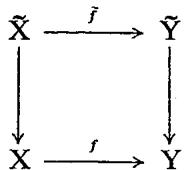
\includegraphics[keepaspectratio]{images/part001_3e847d2c.jpg}}

and compatible with the action of the group \(\{\pm1\}\) .

If \(\tilde{f}\) is an orientation of f and if \(\eta\) is an orientation of Y, there exists one and only one orientation \(\xi\) of X such that the diagram

\pandocbounded{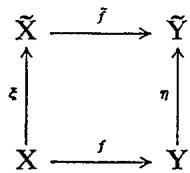
\includegraphics[keepaspectratio]{images/part001_a1f56317.jpg}}

is commutative. We say that \(\xi\) is associated with \(\eta\) by \(f\) .

Examples

\begin{enumerate}
\def\labelenumi{\alph{enumi})}
\item
  If Y is reduced to a point, an orientation of f is equivalent to an orientation of X.
\item
  Suppose \(f\) is étale. For every \(x \in X\), the map \(\mathrm{T}_{x}(f)\) is an isomorphism of \(\mathrm{T}_{x}(\mathrm{X})\) onto \(\mathrm{T}_{f(x)}(\mathrm{Y})\), and defines (by transport of structure) a bijection
\end{enumerate}

\[
\tilde {f} _ {x}: \mathrm{Or} (\mathrm{T} _ {x} (\mathrm{X})) \rightarrow \mathrm{Or} (\mathrm{T} _ {f (x)} (\mathrm{Y})).
\]

The family of \(\tilde{f}_{x}\) defines an orientation \(\tilde{f}\colon\tilde{\mathbf{X}}\to\tilde{\mathbf{Y}}\) of \(f\) , said to be canonical.

\begin{enumerate}
\def\labelenumi{\alph{enumi})}
\setcounter{enumi}{2}
\tightlist
\item
  More generally, suppose that \(f\) is a submersion, and let \(\alpha\) be an orientation of the bundle T(X/Y) (8.1.3). Let \(x\in X\) and \(\xi\) be an orientation of \(\mathrm{T}_{x}(\mathrm{X}/\mathrm{Y})\). Set \(y=f(x)\); we have an exact sequence (8.1.3)
\end{enumerate}

\[
0 \rightarrow \mathrm{T} _ {x} (\mathrm{X} / \mathrm{Y}) \rightarrow \mathrm{T} _ {x} (\mathrm{X}) \xrightarrow {\mathrm{T} _ {x} (f)} \mathrm{T} _ {y} (\mathrm{Y}) \rightarrow 0
\]

and there therefore exists one and only one orientation \(\tilde{f}_{\alpha}(\xi)\) of \(\mathrm{T}_{y}(\mathrm{Y})\) such that \(\xi = \tilde{f}_{\alpha}(\xi)\alpha(x)\) (10.2.1). The map \(\tilde{f}_{\alpha}\colon \tilde{\mathrm{X}}\to \tilde{\mathrm{Y}}\) is an orientation of \(f\), said to be associated with \(\alpha\). The map \(\alpha \mapsto \tilde{f}_{\alpha}\) is a bijection from the set of orientations of \(\mathrm{T}(\mathrm{X}/\mathrm{Y})\) onto the set of orientations of \(f\).

\begin{enumerate}
\def\labelenumi{\alph{enumi})}
\setcounter{enumi}{3}
\tightlist
\item
  If \(f: X \to Y\) is an immersion, the orientations of \(f\) correspond to the orientations of the normal bundle to \(f\) .
\end{enumerate}

10.2.6 ("Orientation of a product"). Let \(\mathbf{X}_1\) (resp. \(\mathbf{X}_2\)) be a manifold locally of finite dimension and \(\xi_1\) (resp. \(\xi_2\)) an orientation of \(\mathbf{X}_1\) (resp. \(\mathbf{X}_2\)). Let \(\mathbf{X} = \mathbf{X}_1 \times \mathbf{X}_2\). The map \((x_1, x_2) \mapsto \xi_1(x_1)\xi_2(x_2)\) (10.2.1) is an orientation of \(\mathbf{X}_1 \times \mathbf{X}_2\), called the product of the orientations \(\xi_1\) and \(\xi_2\), and denoted \(\xi_1\xi_2\), or \(\xi_1 \otimes \xi_2\).

Suppose that \(X_{i}\) (i = 1, 2) are pure of dimension \(n_{i}\). The canonical isomorphism \(X_{1} \times X_{2} \to X_{2} \times X_{1}\) transforms \(\xi_{1} \otimes \xi_{2}\) into \(\xi_{2} \otimes \xi_{1}\) (resp. into \(-\xi_{2} \otimes \xi_{1}\)) if one of the \(n_{i}\) is even (resp. if \(n_{1}\) and \(n_{2}\) are odd).

10.2.7 (“Complex case”). Let F be a finite-dimensional complex vector space and let \(F_{R}\) be the underlying real vector space. Let \(\{e_{1},\ldots,e_{m}\}\) be a basis of F; then \(\{e_{1},ie_{1},e_{2},ie_{2},\ldots,e_{m},ie_{m}\}\) is a basis of \(F_{R}\) and the orientation of \(F_{R}\) defined by the 2m-vector

\[
e _ {1} \wedge i e _ {1} \wedge e _ {2} \wedge i e _ {2} \wedge \dots \wedge e _ {m} \wedge i e _ {m}
\]

is independent of the choice of the basis \(\{e_{1},\ldots,e_{m}\}\) of F; this is called the orientation of \(F_{R}\) defined by the given complex structure. If F is the direct sum of two subspaces G and H, the orientation of \(F_{R}=G_{R}\oplus H_{R}\) is the product of the orientations of \(G_{R}\) and \(H_{R}\) .

Let X be a real manifold locally of finite dimension, equipped with an almost complex structure (8.8.3). For every \(x \in X\) let \(\xi(x)\) be the orientation of \(\mathrm{T}_{x}(\mathrm{X})\) defined by its complex structure. The map \(x \mapsto \xi(x)\) is an orientation of X, called the orientation defined by the almost complex structure. In particular, we shall equip the real analytic manifold X underlying a complex analytic manifold \(X^{c}\) , locally of finite dimension, with the orientation defined by the associated almost complex structure (8.8.6). If one replaces the given complex analytic manifold structure on X by its conjugate (5.4.12.b)), this orientation is multiplied by the function \(x \mapsto (-1)^{\dim_{x} X^{c}}\) .

10.2.8. Examples

\begin{enumerate}
\def\labelenumi{\alph{enumi})}
\tightlist
\item
  Let E be a finite-dimensional real vector space. The real analytic manifold defined by E (5.2.2) is orientable. More precisely, the map \(\xi \mapsto \xi(0)\) is a bijection from the set of orientations of this manifold onto Or(E).
\end{enumerate}

In particular, the manifold \(R^{n}\) has a canonical orientation \(\xi^{n}\) defined by the half-line \(R_{+}e_{1}\wedge\cdots\wedge e_{n}\) of \(\mathrm{Or}(\mathbf{R}^{n})\).

\begin{enumerate}
\def\labelenumi{\alph{enumi})}
\setcounter{enumi}{1}
\item
  Let X be a sphere with center 0 and radius \(\rho\) in \(\mathbf{R}^n\); it is a submanifold of \(\mathbf{R}^n\). For every \(x \in \mathbf{X}\), the space \(\mathbf{T}_x(\mathbf{R}^n) = \mathbf{R}^n\) is the direct sum of the line \(\mathbf{R}x\) and of the hyperplane \(\mathbf{T}_x(\mathbf{X})\). Let \(\eta_x\) be the orientation \(\mathbf{R}_+x\) of \(\mathbf{R}x\) (“outward normal”) and let \(\xi_x\) be the unique orientation of \(\mathbf{T}_x(\mathbf{X})\) such that the product of \(\eta_x\) and \(\xi_x\) is the orientation \(\xi^n\) of \(\mathbf{R}^n\). The map \(x \mapsto \xi_x\) is an orientation of \(\mathbf{X}\), said to be canonical.
\item
  Let X be a connected manifold, and let G be a discrete group acting properly and freely on X. For X/G to be orientable, it is necessary and sufficient that X be orientable and that the action of G on the set of orientations of X be trivial.
\item
  Real projective space \(\mathbf{P}_{n-1}(\mathbf{R})\) is identified with the quotient of the sphere \(S_{n-1}\) by the group \(\{\pm1\}\) acting by \(x\mapsto\pm x\) ; it is orientable if n is even, and non-orientable if n is odd.
\item
  Every quotient of a Lie group by a connected Lie subgroup is orientable.
\end{enumerate}

\subsection{M-twisted differential forms}

10.3.1. Let X be a real manifold of class \(C^{r}\) and let M be a vector bundle with base X, of finite rank and of class \(C^{k}\), with \(0 \leqslant k \leqslant r\). Let \(\lambda_{\mathrm{M}} = (\mathrm{Or}_{\mathrm{M}}, \{\pm 1\}, \mathrm{X}, \pi)\) be the principal fibration associated with the manifold of orientations of M (10.2.2). Let the structural group \(\{\pm 1\}\) act on R by multiplication. We denote by \(\tilde{R}_{M}\) the bundle associated with \(\lambda_{M}\) of fiber type R (endowed with the operation law defined above) (6.5.1); it is equipped (7.10.2) with a vector bundle structure over the base X, of rank 1 and class \(C^{k}\); it is called the bundle of M-twisted scalars.

10.3.2. We have a commutative diagram:

\pandocbounded{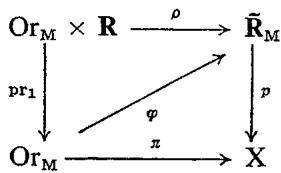
\includegraphics[keepaspectratio]{images/part001_9c73fb1b.jpg}}

where \(p\) denotes the canonical projection of \(\tilde{\mathbf{R}}_{\mathbf{M}}\) onto \(\mathbf{X}\), \(\rho\) the frame map (6.5.1) of \(\tilde{\mathbf{R}}_{\mathbf{M}}\), and where \(\varphi(\xi) = \rho(\xi, 1)\) for \(\xi \in \mathrm{Or}_{\mathbf{M}}\). In particular, the inverse image of the bundle \(\tilde{\mathbf{R}}_{\mathbf{M}}\) by \(\pi\) is identified with the trivial bundle \(\mathrm{Or}_{\mathbf{M}} \times \mathbf{R}\). One also identifies an element \(\xi\) of \(\mathrm{Or}_{\mathbf{M}}\) with its image in \(\tilde{\mathbf{R}}_{\mathbf{M}}\) by \(\varphi\); with this convention, one has \(\rho(\xi, a) = a\xi\) for all \((\xi, a) \in \mathrm{Or}_{\mathbf{M}} \times \mathbf{R}\); we have \(a\xi = b\eta\) if and only if there exists \(e \in \{\pm 1\}\) such that \(b = ea\) and \(\eta = e\xi\). An orientation \(\xi\) of \(\mathbf{M}\) thus defines a section \(x \mapsto \xi(x)\) of \(\tilde{\mathbf{R}}_{\mathbf{M}}\).

There exists one and only one isomorphism \(j\) from \(\tilde{\mathbf{R}}_{\mathbf{M}} \otimes \tilde{\mathbf{R}}_{\mathbf{M}}\) onto the trivial bundle \(\mathbf{R}_{\mathbf{x}} = \mathbf{X} \times \mathbf{R}\) such that \(j(\xi \otimes \xi) = (\pi(\xi), 1)\) for all \(\xi \in \mathrm{Or}_{\mathbf{M}}\); this allows one to identify the vector bundle \(\tilde{\mathbf{R}}_{\mathbf{M}}\) with its dual.

10.3.3. Let F moreover be a vector bundle over the base X and of class \(C^{r-1}\). A differential form on X with values in \(\tilde{R}_{M} \otimes F\) is called an M-twisted differential form with values in F. Such a form of degree p is a section of the bundle \(\operatorname{Alt}^{p}(\mathrm{T}(\mathrm{X}); \tilde{\mathbf{R}}_{\mathbf{M}} \otimes \mathbf{F})\), which one identifies in the obvious way with \(\tilde{R}_{M} \otimes \operatorname{Alt}^{p}(\mathrm{T}(\mathrm{X}); \mathbf{F})\). When F is the trivial bundle defined by a Banach space E, one speaks simply of an M-twisted form with values in E; when E = C (resp. R), one says complex M-twisted form (resp. real M-twisted form, or M-twisted form).

Let \(\omega\) be an M-twisted form of degree \(p\) with values in F. The fact that \(\pi\colon\mathrm{Or}_{\mathbb{M}}\to\mathbf{X}\) is étale and that \(\pi^{*}(\tilde{\mathbf{R}}_{\mathbb{M}})=\mathrm{Or}_{\mathbb{M}}\times\mathbf{R}\) allows one to identify \(\pi^{*}(\tilde{\mathbf{R}}_{\mathbb{M}}\otimes\operatorname{Alt}^{p}(\mathrm{T}(\mathrm{X});\mathrm{F}))\) with \(\mathrm{Alt}^{p}(\mathrm{T}(\mathrm{Or}_{\mathbb{M}});\pi^{*}(\mathrm{F}))\), and \(\omega\) defines a section \(\tilde{\omega}\) of \(\mathrm{Alt}^{p}(\mathrm{T}(\mathrm{Or}_{\mathbb{M}});\pi^{*}(\mathrm{F}))\) (7.4.3), in other words, a differential form of degree \(p\) on \(\mathrm{Or}_{\mathbb{M}}\) with values in \(\pi^{*}(\mathrm{F})\). This yields a bijection from the space of M-twisted forms of degree \(p\) on X with values in F onto the space of forms \(\tilde{\omega}\) of degree \(p\) on \(\mathrm{Or}_{\mathbb{M}}\) with values in \(\pi^{*}(\mathrm{F})\) such that

\[
\tilde{\omega}(-\xi)=-\tilde{\omega}(\xi)\quad\text{for every }\xi\in\mathrm{Or}_{\mathbb{M}}.
\]

When M is equipped with an orientation \(\xi\), the map \(\omega \mapsto \xi \otimes \omega\) makes it possible to identify the sections of \(\mathrm{Alt}^p(\mathrm{T}(\mathrm{X});\mathrm{F})\) (in other words, the usual differential forms of degree \(p\)) with M-twisted forms of degree \(p\) with values in F.

10.3.4. Let \(\omega\) be an M-twisted differential form of degree \(p\) on X, with values in a Banach space E, and of class \(\mathbf{C}^s\) (\(1 \leqslant s \leqslant \inf(k, r - 1)\)). There exists one and only one M-twisted differential form \(d\omega\), of degree \(p + 1\) on X, with values in E, such that, for every open set U of X, every orientation \(\xi\) of \(M|_{U}\), and every differential form \(\alpha\) on U such that \(\omega|_{U} = \xi \otimes \alpha\), one has \(d\omega|_{U} = \xi \otimes d\alpha\). The form \(d\omega\) is of class \(\mathbf{C}^{s-1}\); it is called the exterior differential of \(\omega\).

If one denotes by \(\tilde{\omega}\) (resp. \(\widetilde{d\omega}\)) the differential form on \(\mathrm{Or}_{\mathbb{M}}\) corresponding to \(\omega\) (respectively to \(d\omega\)) as in 10.3.3, one has \(d(\tilde{\omega}) = \widetilde{d\omega}\).

If \(\zeta\) is a vector field of class \(\mathbf{C}^s\) onto \(X\) , one defines in an analogous manner the M-twisted form \(\theta_{\zeta}.\omega\) . One has

\[
\theta_ {\zeta}. \omega = d (i (\zeta) \omega) + i (\zeta) d \omega
\]

and \(\theta_{\zeta}.\omega\) is of class \(\mathbf{C}^{s - 1}\).

\subsection{Measure associated with a twisted differential form}

Recall that, in this section, we assume K = R and that all manifolds considered are locally finite-dimensional.

10.4.1. Let X be a manifold of class \(C^{r}\). One can apply the definitions and results of 10.3 by taking as vector bundle M the tangent bundle T(X). One then has \(\mathrm{Or}_{\mathbf{M}} = \tilde{\mathbf{X}}\) (10.2.4); we denote it by \(\tilde{\mathbf{R}}_{\mathbf{X}}\) and call simply the bundle of twisted scalars the bundle \(\tilde{\mathbf{R}}_{\mathrm{T}(\mathbf{X})}\) (10.3.1)\footnote{Note that this notation conflicts with the notation \(\widetilde{\mathbf{R}}_{\mathbf{M}}\) when X is regarded as endowed with its vector-bundle structure of rank 0 over itself.}; a T(X)-twisted differential form with values in a vector bundle F is called simply a twisted (or odd) differential form with values in F. When X is equipped with an orientation, the map \(\omega \mapsto \xi \otimes \omega\) allows one to identify the usual differential forms (sometimes called "even") with the twisted forms.

10.4.2. Let \(f\colon\mathbf{X}\to\mathbf{Y}\) be a morphism of manifolds of class \(\mathbf{C}^{r}\) and let \(\tilde{f}\colon\tilde{\mathbf{X}}\to\tilde{\mathbf{Y}}\) be an orientation of \(f\) (10.2.5). There exists one and only one isomorphism \(j\) from \(f^{*}(\widetilde{\mathbf{R}}_{\mathbf{Y}})\) onto \(\widetilde{\mathbf{R}}_{\mathbf{X}}\) such that \(\tilde{x}=j(\pi(\tilde{x}),\tilde{f}(\tilde{x}))\) for all \(\tilde{x}\in\tilde{\mathbf{X}}\). We identify these two bundles by means of \(j\). If \(\omega\) is a twisted form of degree \(p\) on Y with values in a vector bundle F, the inverse image \(f^{*}(\omega)\) is identified with a twisted differential form of degree \(p\) on X with values in \(f^{*}(\mathrm{F})\). If one denotes by \(\tilde{\omega}\) (resp. \(\widetilde{f^{*}(\omega)}\)) the differential form on \(\tilde{\mathbf{Y}}\) (resp. \(\tilde{\mathbf{X}}\)) corresponding to \(\omega\) (resp. \(f^{*}(\omega)\)) as in 10.3.3, one has \(\tilde{f}^{*}(\tilde{\omega})=\widetilde{f^{*}(\omega)}\).

When F is the trivial bundle defined by a Banach space, the operation \(f^*\) commutes with exterior differentiation (10.3.4).

10.4.3. Let X be a pure manifold of dimension n, and let \(\omega\) be a twisted differential form of degree n on X, with values in a Banach space E. Let \(c = (\mathrm{U}, \varphi, \mathbf{R}^{n})\) be a chart of X and let \(\xi^{n}\) be the canonical orientation of \(R^{n}\); denote by \(u^{1}, \ldots, u^{n}\) the coordinate functions on \(R^{n}\). There exists one and only one function \(f_{c}\) on \(\varphi(\mathrm{U})\), with values in E, such that

\[
\omega | \mathrm{U} = \varphi^ {*} (\xi^ {n} \otimes f _ {c}. d u ^ {1} \wedge \dots \wedge d u ^ {n}).
\]

One says that \(\omega\) is locally integrable if, for every chart \(c = (\mathrm{U},\varphi ,\mathbb{R}^n)\) of X, the corresponding function \(f_{c}\) is locally integrable with respect to \(\lambda_{\varphi (\mathrm{U})}^{\otimes n}\) (where \(\lambda\) denotes Lebesgue measure on R). Suppose that this is the case and that X is separated. There exists on X a vector measure \(\alpha (\omega)\) with values in E and one and only one possessing the following property: for every chart \(c = (\mathrm{U},\varphi ,\mathbb{R}^n)\) of X, the image under \(\varphi\) of the restriction to U of the measure \(\alpha (\omega)\) is the measure \(f_{c}\lambda_{\varphi(\mathrm{U})}^{\otimes n}\) (INT, VI, § 2, no. 4). One says that \(\alpha (\omega)\) is the measure defined by \(\omega\) and one denotes it most often simply by \(\omega\). The support of \(\alpha (\omega)\) is contained in the support \(\operatorname{Supp}\omega\) of \(\omega\) (calling the support of a differential form \(\omega\) the closure of the set of \(x\in X\) such that \(\omega (x)\neq 0\)).

If \(f\) is a real function on X, locally integrable with respect to the measure \(\alpha(\omega)\), then the differential form \(f\omega\) is locally integrable and one has \(\alpha(f\omega) = f.\alpha(\omega)\).

If \(g\) is a real function on X essentially integrable for \(\alpha(\omega)\), its integral is generally denoted \(\int_{\mathbf{X}} g\omega\), or \(\int g\omega\), or \(\int g(x)\omega(x)\); one avoids denoting it \(\int g d\omega\), because of the risk of confusion with the exterior differential \(d\omega\) of \(\omega\), which is defined (and moreover equal to 0) if \(\omega\) is of class \(C^{1}\). If A is a subset of X whose characteristic function \(\varphi_{\mathrm{A}}\) is essentially integrable for \(\alpha(\omega)\), the integral of \(\varphi_{\mathrm{A}}\) is denoted \(\int_{A} \omega\). If the constant 1 is essentially integrable for \(\alpha(\omega)\), one says that \(\omega\) is integrable.

Now let \(p\) be an integer, with \(0 \leqslant p \leqslant n\), and let \(\omega\) be a twisted differential form of degree \(p\) on X, with values in a Banach space E. Let moreover Y be a pure submanifold of dimension \(p\) of X; suppose that the canonical injection \(i: Y \to X\) is equipped with an orientation. The inverse image \(i^{*}(\omega)\) (10.4.2) is then sometimes denoted \(\omega|Y\). If \(\omega|Y\) is integrable, we set

\[
\int_ {\mathbf {Y}} \omega = \int_ {\mathbf {Y}} \omega | \mathbf {Y}.
\]

10.4.4. Let X be a pure manifold of dimension n, equipped with an orientation \(\xi\). The identification \(\omega \mapsto \xi \otimes \omega\) between usual differential forms and twisted differential forms makes it possible to apply the preceding results to forms of degree n on X; thus, to every locally integrable form \(\omega\) of degree n, there is associated a measure on X, still denoted \(\omega\). If E = R, such a form \(\omega\) is locally of integrable modulus (10.1.5) and the measure \(\text{mod}(\omega)_{\mu}\) corresponding to it (10.1.6) is none other than the absolute value \(|\omega|\) of the measure \(\omega\) (INT, III, § 1, no. 6).

10.4.5. Example. --- Let X be a pure real manifold of dimension 1, oriented, separated, and let \(z: \mathrm{X} \to \mathbf{C}\) be a differentiable map from X to C. The complex differential form \(dz\) defines on X a complex measure also denoted \(dz\) . This applies in particular when X is a pure differentiable submanifold of dimension 1 of C, \(z\) being the injection of X into C.

More specifically, let X be a circle with center 0 and radius \(\rho > 0\); orient X as indicated in 10.2.8, b), given the usual identification of C with \(\mathbf{R}^2\). If \(x \in \mathbf{X}\), the tangent space \(\mathrm{T}_x(\mathbf{X})\) is identified with the line \(\mathbf{R}ix\) of \(\mathrm{T}_x(\mathbf{C}) = \mathbf{C}\), and the chosen orientation is the half-line \(\mathbf{R}_+ix\). If \(f\) is a continuous function on X, with values in a complex Banach space, the integral of \(f\) for the measure \(dz\) is given by the formula

\[
\int_ {\mathbb {X}} f (z) d z = i \rho \int_ {0} ^ {2 \pi} f (\rho e ^ {i \alpha}) e ^ {i \alpha} d \alpha .
\]

For example, if \(n\) is an integer, we have

\[
\int_ {\mathrm{X}} z ^ {n} d z = i \rho^ {n + 1} \int_ {0} ^ {2 \pi} e ^ {(n + 1) i \alpha} d \alpha = \left\{ \begin{array}{l l} 0 & \quad \text {if } n \neq - 1 \\ 2 i \pi & \quad \text {if } n = - 1. \end{array} \right.
\]

10.4.6 (“Complex case”). Let \(X^{c}\) be a separated complex analytic manifold, pure of dimension \(m\), and let \(\omega\) be a holomorphic differential form of degree \(m\) on \(X^{c}\). Let X be the real analytic manifold underlying \(X^{c}\); the form \(\omega\) identifies with a form of type \((m,0)\) on X (8.8.9); let \(\overline{\omega}\) be its conjugate (8.8.2). The form \(i^{m^{2}}\omega \wedge \overline{\omega}\) is a real differential form of degree \(2m\) on X; taking into account the canonical orientation of X (10.2.7), this form identifies with a measure on X, which is none other than the positive measure \(\operatorname{mod}(\omega)_{\mu}\) defined in 10.1.6, where \(\mu\) is the measure defined by the differential form \(i \, dz \wedge \overline{dz}\), in other words twice the Lebesgue measure \(\lambda^{\otimes 2}\) on \(\mathbf{C}\) (identified with \(\mathbf{R}^{2}\) in the usual way).

Let H be the space of holomorphic forms \(\omega\) of degree \(m\) on \(\mathbf{X}^c\) such that the measure \(\omega \wedge \overline{\omega}\) is bounded. For \(\alpha, \beta\) in H, the complex measure \(\alpha \wedge \overline{\beta}\) is bounded; setting

\[
(\alpha | \beta) = i ^ {m ^ {2}} \int_ {\mathbf {X}} \alpha \wedge \bar {\beta},
\]

one obtains a Hermitian form on H, which makes H into a Hilbert space.

\section{Stokes' formula}

In this paragraph, we assume K = R.

\subsection{Pieces}

11.1.1. Let E be a Banach space. A subset S of E is called a closed half-space if there exists a continuous linear functional \(h \neq 0\) and a real number k such that \(S = \{x|h(x) \leqslant k\}\) (cf. EVT, II, §2, no. 6); the boundary of S is then the closed hyperplane \(\{x|h(x) = k\}\) ; it is also called the boundary of S, and is denoted by \(\partial S\) .

11.1.2. Let X be a manifold of class \(C^{r}\) and A a subset of X. One says that A is a piece of X if, for every \(a \in A\), there exists a chart \(c = (U, \varphi, E)\) of X at a such that \(\varphi(A \cap U)\) is an open subset of a closed half-space of E. We set \(\partial A = A - \mathring{A}\) (the set of non-interior points of A). It is a submanifold of A, called the boundary of A.\footnote{This terminology comes from the fact that A is naturally endowed with a structure of a “manifold with boundary”, with boundary \(\partial A\). For the definition of this category, as well as for the more general category of “manifolds with corners”, the reader may consult H. Cartan, \emph{Séminaire 1961/62, Topologie Différentielle}, lectures 1–2–3 (by A. Douady), Benjamin, New York, 1969. Let us mention that one can show that every “manifold with boundary” whose boundary is paracompact is isomorphic to a closed piece of a manifold.} If \(a \in \partial A\), there exists a chart \(c = (U, \varphi, E)\) of X centered at a and a closed hyperplane H of E such that \(\varphi(A \cap U)\) is an open neighborhood of 0 in one of the closed half-spaces \(S_{c}\) of E defined by H (EVT, II, § 2, no. 6), and \(\varphi(\partial A \cap U) = H \cap \varphi(A \cap U)\). Such a chart is said to be adapted to A at a. The closed half-space \(S_{c}\) is then the unique closed half-space of E for which \(\varphi(A \cap U)\) is an open set.

For a closed subset A of X to be a piece of X, it is necessary and sufficient that \(\mathring{A}\) be dense in A and that \(A-\mathring{A}\) be a submanifold of X of codimension 1 at each of its points.

11.1.3. Examples

\begin{enumerate}
\def\labelenumi{\alph{enumi})}
\item
  In \(\mathbf{R}^{n}\) a closed ball of radius \(>0\) is a piece; its boundary is the corresponding sphere.
\item
  If A is a piece of the manifold X and if B is a closed subset of \(\partial A\) then A - B is a piece of X.
\item
  Let \(\varphi: X \to X'\) be a morphism of manifolds of class \(C^r\) , and let \(A'\) a piece of \(X'\) . If \(\varphi\) is transverse to \(\partial A'\) (5.11.6), \(\varphi^{-1}(A')\) is a piece of \(X\) whose boundary is \(\varphi^{-1}(\partial A')\) .
\end{enumerate}

In particular, let \(h: \mathbf{X} \to \mathbf{R}\) be a function of class \(\mathbf{C}^r\) , and let \(a \in \mathbf{R}\) ; suppose that there exists no \(x \in \mathbf{X}\) such that \(h(x) = a\) and \(d_x h = 0\) . The set \(\{x | h(x) \leqslant a\}\) is a closed piece of \(\mathbf{X}\) with boundary \(h^{-1}(a)\) .

\begin{enumerate}
\def\labelenumi{\alph{enumi})}
\setcounter{enumi}{3}
\tightlist
\item
  If \(r = \infty\) and if X is locally compact, every compact subset of X admits a fundamental system of neighborhoods consisting of compact pieces.
\end{enumerate}

11.1.4. Let X be a manifold of class \(\mathbf{C}^{\mathrm{r}}\) and let A be a piece of X. Let \(a \in \partial \mathrm{A}\) and \(v \in \mathrm{T}_a(\mathrm{X})\) . Let \(c = (\mathrm{U}, \varphi, \mathrm{E})\) be a chart of X adapted to A at \(a\) (11.1.2), and let \(h = \theta_c^{-1}(v)\) be the element of E corresponding to \(v\) (5.5.1). Let \(\mathrm{S}_c\) be the closed half-space of E of which \(\varphi(\mathrm{A} \cap \mathrm{U})\) is an open subset (11.1.2). One says that \(v\) is an inward (resp. strictly inward, resp. outward, resp. strictly outward) vector for A at \(a\) if \(h\) belongs to \(\mathrm{S}_c\) (resp. \(\dot{\mathrm{S}}_c\) , \(-\mathrm{S}_c\) , \(-\dot{\mathrm{S}}_c\) ), a condition which is independent of the choice of the adapted chart \(c\) . We denote by \(\mathrm{T}_a^+(\mathrm{A})\) (resp. \(\mathrm{T}_a^-(\mathrm{A})\) ) the set of outward (resp. inward) vectors of \(\mathrm{T}_a(\mathrm{X})\) for A. These are closed half-spaces of \(\mathrm{T}_a(\mathrm{X})\) , whose boundary contains 0. One has

\[
\mathrm{T} _ {a} (\partial \mathrm{A}) = \mathrm{T} _ {a} ^ {+} (\mathrm{A}) \cap \mathrm{T} _ {a} ^ {-} (\mathrm{A}).
\]

\subsection{Stokes' formula for pieces}

In this section, X denotes a manifold of class \(C^{r}\) ( \(r \geqslant 2\) ) pure of finite dimension n and separated. A denotes a piece of X and i the canonical injection of \(\partial A\) into X. E denotes a Banach space.

11.2.1. Let \(x \in \partial A\) and let \(\xi\) be an orientation of \(T_x(\partial A)\); one denotes \(\tilde{i}_x(\xi)\) the orientation of \(T_x(X)\) containing the elements \(v \wedge u\), where \(v\) is a strictly outward vector for A at x (11.1.4) and where \(u\) is a nonzero element of \(\bigwedge^{n-1} T_x(\partial A)\) belonging to the orientation \(\xi\). The map \(\tilde{i}_x\) is a bijection of \(\text{Or}(T_x(\partial A))\) onto \(\text{Or}(T_x(X))\). The maps \(\tilde{i}_x\), for \(x \in \partial A\), define a morphism \(\tilde{i} \colon \partial \widetilde{A} \to \widetilde{X}\) which is an orientation of \(i\) (10.2.5). If \(\xi\) is an orientation of X, the orientation of \(\partial A\) associated with \(\xi\) by \(\tilde{i}\) (10.2.5) is said to be defined by \(\xi\).

Example. --- When \(X = R^{n}\), \(\xi\) is the usual orientation of \(R^{n}\), and A is a closed ball of radius \(\rho>0\), the orientation of the sphere \(\partial A\) defined by \(\xi\) is the canonical orientation (10.2.8, b)).

11.2.2. Let \(\omega\) be a twisted differential form of degree \(p\) on X with values in a Banach space E (10.4.1); the inverse image \(i^{*}(\omega)\) of \(\omega\) by the oriented morphism \(i\colon\partial A\to X\) is denoted \(\omega|\partial A\) and is called the form induced by \(\omega\) on \(\partial A\) (cf. 10.4.3).

11.2.3. Let us make one of the following two assumptions:

\begin{enumerate}
\def\labelenumi{(\roman{enumi})}
\tightlist
\item
  \(\omega\) is a twisted differential form of degree \(n - 1\) on X, with values in E;
\item
  X is oriented, \(\partial A\) is equipped with the corresponding orientation (11.2.1), and \(\omega\) is a differential form of degree \(n - 1\) on X with values in E.
\end{enumerate}

Suppose moreover that \(\omega\) is of class \(C^{1}\) and that the intersection of A and the support of \(\omega\) is compact. The exterior differential \(d\omega\) of \(\omega\) is continuous (8.3.5 and 10.3.4).

The characteristic function of A is essentially integrable with respect to the vector measure defined by \(d\omega\) on X, and the differential form \(\omega|\partial\mathrm{A}\) of degree \(n-1\) on \(\partial\mathrm{A}\) is integrable (10.4.3 and 10.4.4). We have

\[
\int_ {\mathrm{A}} d \omega = \int_ {\partial \mathrm{A}} \omega \quad (\text{Stokes' formula})
\]

11.2.4. Let \(\alpha\) be a twisted differential form of degree \(n\) on X with values in a Banach space E, with compact support and of class \(\mathbf{C}^1\). For there to exist a twisted differential form \(\omega\) of degree \(n - 1\) on X, with values in E, with compact support and of class \(\mathbf{C}^1\), such that \(\alpha = d\omega\), it is necessary that \(\int_{\mathbb{X}} \alpha = 0\). If X is connected, this condition is sufficient; if moreover \(\alpha\) is of class \(\mathbf{C}^k\) (\(k\leqslant r-1,\ k\neq\omega\)), one can choose \(\omega\) of class \(\mathbf{C}^k\).

11.2.5. Suppose that X is the real manifold underlying \(\mathbf{C}\), that E is a complex Banach space, and that A is a compact piece of X. Endow X with the orientation defined by its complex structure (10.2.7). Let f be a continuous map from A into E whose restriction to the interior \(\mathring{A}\) of A is holomorphic. Denote by \(dz\) the differential of the injection \(z\colon\partial A\to\mathbf{C}\). The form \(f\cdot dz\), the product of f and dz, is a differential form of degree 1 on \(\partial A\), with values in E, of class \(C^{0}\), and one has:

\[
\int_ {\partial \mathbf {A}} f\, d z = 0 \quad (\text{Cauchy's formula})
\]

When \(f\) extends to a holomorphic map, still denoted \(f\), from an open neighborhood U of A into E, the differential form \(f.dz\) (where z now denotes the canonical injection of U into \(\mathbf{C}\)) is of class \(C^{\omega}\) on U and its exterior differential is zero.

11.2.6 (“Derivative of an integral”). Suppose X is oriented. Let Y be a manifold of class \(C^{r}\), and let \(\alpha\) be a differential form of degree \(n\) on Y, with values in E, of class \(C^{1}\), and with compact support. Let I be an open subset of R containing 0, and let \(g: I \times X \to Y\) be a morphism of class \(C^{r}\); for \(t \in I\), denote by \(g_{t}\) the map \(x \mapsto g(t, x)\) from X into Y. Denote by \(\psi\) the morphism from X into T(Y) defined by \(\psi(x) = T_{(0,x)}(g)(1,0)\); it is a lifting of \(g_{0}\) (8.6.5). Suppose that the restriction of \(\operatorname{pr}_{1}\colon I\times A\to I\) to the intersection of \(I\times A\) and the support of \(g^{*}(\alpha)\) is proper (TG, I, § 10). For every \(t \in I\), the intersection of A and the support of \(g_{t}^{*}(\alpha)\) is then compact; the map \(t \mapsto \int_{A} g_{t}^{*}(\alpha)\) is of class \(C^{1}\) on I and its derivative at the origin is given by the formula

\[
\frac {d}{d t} \left(\int_ {\mathrm{A}} g _ {t} ^ {*} (\alpha)\right) _ {t = 0} = \int_ {\mathrm{A}} \theta_ {\psi}. \alpha = \int_ {\mathrm{A}} i (\psi) d \alpha + \int_ {\partial \mathrm{A}} i (\psi) \alpha ,
\]

cf. no. 8.6.

\subsection{Stokes' formula for locally polyhedral sets}

In this number, X denotes a pure real manifold of finite dimension n of class \(C^{r}\) ( \(r \geqslant 2\) ); we assume X is separated.\footnote{The reader interested in more general cases may consult H. Whitney, \emph{Geometric Integration Theory}, Chap. III, § 18 (Princeton Univ. Press, 1957).}

11.3.1. Let A be a subset of a finite-dimensional real vector space. We say that A is polyhedral if it is a finite union of finite intersections of closed half-spaces.

A subset A of X is said to be locally polyhedral if, for every \(x \in X\), there exists a chart \(c = (\mathrm{U}, \varphi, \mathrm{E})\) of X at x and a polyhedral subset \(A_{c}\) of E such that \(\varphi(\mathrm{A} \cap \mathrm{U}) = \varphi(\mathrm{U}) \cap \mathrm{A}_{c}\). A piece of X is a locally polyhedral subset.

11.3.2. Let A be a closed subset of X, and let \(\mathrm{Fr}(\mathrm{A}) = \mathrm{A} - \mathring{\mathrm{A}}\) be its frontier. A point \(x \in \mathrm{Fr}(\mathrm{A})\) is said to be regular if there exists an open neighborhood U of x such that \(A \cap U\) is a piece of the manifold U (in which case x belongs to the boundary of \(A \cap U\)). We denote by \(\partial A\) the set of regular points of \(\mathrm{Fr}(\mathrm{A})\) and call it the regular boundary (or simply the boundary) of A. The set \(A' = \mathring{A} \cup \partial A\) is a piece of X, with boundary \(\partial A\).

11.3.3. * Example. --- Let \(\mathcal{H}\) be a locally finite set of hyperplanes of a finite-dimensional real affine space E of dimension \(n\), and let C be a chamber of E relative to \(\mathcal{H}\) (LIE, V, § 1, no. 3). The closure \(\overline{\mathbf{C}}\) of C is a locally polyhedral subset of the manifold E; the regular boundary of \(\overline{\mathbf{C}}\) is the union of the faces of C (loc. cit., no. 4). In particular, if C is an open simplex (loc. cit., no. 6) with vertices \(a_0, \ldots, a_n\), the boundary of \(\overline{\mathbf{C}}\) is the union of the \(\overline{\mathbf{C}_{\{i\}}}\) (\(0 \leqslant i \leqslant n\)), where \(\mathbf{C}_{\{i\}}\) is the open simplex with vertices \(a_0, \ldots, a_{i-1}, a_{i+1}, \ldots, a_n\) in the affine space generated by these vertices.* 
11.3.4. Let A be a locally polyhedral subset of X, and let \(\omega\) be a twisted differential form of degree \(n - 1\) on X with values in a Banach space E; suppose that \(\omega\) is of class \(\mathbf{C}^1\) and that the intersection of its support with A is compact. Then, the characteristic function of A (resp. \(A'\), \(\mathring{A}\)) is essentially integrable for the vector measure defined by \(d\omega\) on X, and one has

\[
\int_ {\mathrm{A}} d \omega = \int_ {\mathrm{A} ^ {\prime}} d \omega = \int_ {\mathring{\mathrm{A}}} d \omega.
\]

The differential form \(\omega|\partial\mathbf{A}\) (for the canonical orientation of the canonical injection of \(\partial\mathbf{A}\), considered as the boundary of the piece \(\mathbf{A}'\), into \(\mathbf{X}\)) is integrable on \(\partial\mathbf{A}\), and one has

\[
\int_ {\mathbf {A}} d \omega = \int_ {\partial \mathbf {A}} \omega \quad (\text{Stokes' formula}).
\]

When X is equipped with an orientation, and \(\partial\mathbf{A}\) is equipped with the corresponding orientation (11.2.1), this formula remains valid if \(\omega\) is an ordinary differential form of degree \(n-1\) with values in E, of class \(\mathbf{C}^{1}\), and such that \(\mathbf{A}\cap\operatorname{Supp}\omega\) is compact.

\subsection{Relative Stokes' formula (integration over the fibers)}

In this number, X and S denote two (real) manifolds of class \(C^{r}\), and \(\pi: X \to S\) a submersion. We denote by n an integer and suppose that, for every \(s \in S\), the fiber \(X_{s} = \pi^{-1}(s)\) of \(\pi\) at s (which is a submanifold of X (5.10.5)) is pure of dimension n.

11.4.1. Let E and H be two vector spaces and let F be a vector subspace of finite dimension n of H.

Let p be an integer \(\geqslant0\), u an alternating \((n+p)\)-linear map from \(H^{n+p}\) into E, and \(t_{1},\ldots,t_{p}\) elements of \(H/F\); let \(t_{1}^{\prime},\ldots,t_{p}^{\prime}\) be representatives of \(t_{1},\ldots,t_{p}\) in H. The map

\[
(x _ {1}, \dots , x _ {n}) \mapsto u (t _ {1} ^ {\prime}, \dots , t _ {p} ^ {\prime}, x _ {1}, \dots , x _ {n})
\]

is an n-linear alternating map from \(\mathbf{F}^n\) into E, which depends only on u and on the \(t_i\); it is denoted \(u \perp (t_1, \ldots, t_p)\) (cf. A, III, p. 158 for the particular case \(\mathbf{E} = \mathbf{K}\)). The map

\[
\left(t _ {1}, \dots , t _ {p}\right) \mapsto u \perp \left(t _ {1}, \dots , t _ {p}\right)
\]

is p-linear alternating.

11.4.2 (“\(\pi\)-twisted”). Consider the vector bundle \(\mathrm{T}(\mathrm{X}/\mathrm{S})\) on X (8.1.3); it has finite rank n at each point of X. We set \(\tilde{R}_{\pi} = \tilde{R}_{T(X/S)}\) (10.3.1) and \(\tilde{X}_{\pi} = \mathrm{Or}_{T(X/S)}\) (10.2.2). Let \(s \in S\); given the natural identification \(\mathrm{T}(\mathrm{X}/\mathrm{S})|_{\mathbf{X}_{s}}\) with \(\mathrm{T}(\mathbf{X}_{s})\) (8.1.3), the fiber at s of the map \(\tilde{\pi}: \tilde{X}_{\pi} \to S\), composite of \(\pi\) and the canonical map \(\tilde{X}_{\pi} \to X\), is \(\tilde{X}_{s}\) (10.2.4). A \(\pi\)-twisted differential form on X is called a \(\mathrm{T}(\mathrm{X}/\mathrm{S})\)-twisted differential form (10.3.3).

11.4.3 (“S-orientation of an S-morphism”). Let \(\mathbf{X}'\) be a variety equipped with a submersion \(\pi'\colon\mathbf{X}'\to\mathbf{S}\) whose fibers \(\mathbf{X}'_{s}\) are pure of finite dimension \(n'\), and let \(\varphi\colon\mathbf{X}'\to\mathbf{X}\) be a morphism such that \(\pi'=\pi\circ\varphi\). An S-orientation of \(\varphi\) is a morphism \(\tilde{\varphi}\colon\tilde{\mathbf{X}}'_{\pi'}\to\tilde{\mathbf{X}}_{\pi}\), commuting with the action of the group \(\{\pm1\}\) and such that the diagram

\pandocbounded{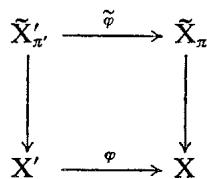
\includegraphics[keepaspectratio]{images/part001_c0391fc0.jpg}}

is commutative. The datum of an S-orientation of \(\varphi\) allows, as in 10.4.2, one to identify the bundles \(\tilde{\mathbf{R}}_{\pi'}\) and \(\varphi^{*}(\tilde{\mathbf{R}}_{\pi})\) and to define the pullback of a \(\pi\)-twisted differential form by the S-oriented morphism \(\varphi\); it is a \(\pi'\)-twisted differential form on \(\mathbf{X}'\).

11.4.4. Let A be a piece of X such that the restriction of \(\pi\) to \(\partial\mathbf{A}\) is a submersion. For every \(s\in\mathbf{S}\), the fiber \(\mathbf{X}_{s}=\pi^{-1}(s)\) is a submanifold of X transverse to \(\partial\mathbf{A}\), and \(\mathbf{A}\cap\mathbf{X}_{s}\) is a piece of \(\mathbf{X}_{s}\), denoted \(\mathbf{A}_{s}\), with boundary \(\partial\mathbf{A}\cap\mathbf{X}_{s}\).

Let \(i\) be the canonical injection of \(\partial\mathbf{A}\) into X. There exists one and only one S-orientation \(\tilde{i}\) of \(i\) such that, for every \(s\in\mathbf{S}\), the restriction of \(\tilde{i}\) to \((\partial\mathbf{A}_{s})^{\sim}\) (identified with the fiber at s of the submersion \(\partial\widetilde{\mathbf{A}}_{\pi|\partial\mathbf{A}}\to\mathbf{S}\)) is the orientation defined in 11.2.1 of the canonical injection of \(\partial\mathbf{A}_{s}\) into \(\mathbf{X}_{s}\). If \(\omega\) is a \(\pi\)-twisted differential form on X, the inverse image of \(\omega\) under the morphism \(i\) thus oriented is denoted \(\omega|\partial\mathbf{A}\) (cf. 11.2.2).

11.4.5 ("Interior product"). Let p be an integer \(\geqslant 0\) and let \(\omega\) be a \(\pi\)-twisted differential form of degree \(n + p\) on X, with values in a vector bundle E with base X. Let \(s \in S\) and \(x \in X_s\); we have \(\omega(x) = \xi \otimes u\), where \(\xi\) is an orientation of \(T_x(X_s) = T(X/S)_x\), identified with an element of \((\tilde{\mathbf{R}}_{X_s})_x = (\tilde{\mathbf{R}}_n)_x\) (10.3.2), and where u is an alternating \((n + p)\)-linear map from \(T_x(X)\) into \(E_x\). Let \(t_1, \ldots, t_p\) be tangent vectors to S at s. Put

\[
\theta (x) = \xi \otimes (u \llcorner (t _ {1}, \dots , t _ {p})) \in (\tilde {\mathbf {R}} _ {\mathrm{X} _ {s}}) _ {x} \otimes (\mathrm{Alt} ^ {n} (\mathrm{T} (\mathrm{X}); \mathrm{E})) _ {x}
\]

(cf. 11.4.1). One thus defines a twisted differential form \(\theta: x \mapsto \theta(x)\) of degree n on \(X_s\), with values in \(E|_{X_{s}}\). We denote it by \(\omega \perp (t_1, \ldots, t_p)\).

In particular, let M be a vector bundle of class \(C^{r-1}\) with base S and take \(E = \pi^{*}(M)\). The bundle \(E|_{X_{s}}\) is naturally identified with the trivial bundle with base \(X_{s}\) defined by the Banach space \(M_{s}\), and the form \(\omega\perp(t_{1},\ldots,t_{p})\) is identified with a twisted differential form on \(X_{s}\), with values in \(M_{s}\).

11.4.6. We keep the preceding notation (in particular \(E=\pi^{*}(M)\)) and assume moreover that X is separated and \(\omega\) is continuous. Let A be a piece of X such that the restriction of \(\pi\) to \(\partial A\) is a submersion and the restriction of \(\pi\) to the intersection of A and the support of \(\omega\) is proper. For \(s \in S\) and \(t_{1},\ldots,t_{p}\in\mathrm{T}_{s}(\mathrm{S})\), the form \(\omega \perp (t_{1}, \ldots, t_{p})\) (11.4.5) is a twisted differential form of degree n on \(X_{s}\), continuous, with values in the Banach space \(M_{s}\), and its support meets \(A_{s}\) in a compact set. There exists one and only one differential form \(\alpha\) of degree p on S, with values in the vector bundle M, and such that

\[
\alpha (s) \left(t _ {1}, \dots , t _ {p}\right) = \int_ {\mathrm{A} _ {s}} \omega \perp \left(t _ {1}, \dots , t _ {p}\right)
\]

for all \(s \in S\) and \(t_{1},\ldots,t_{p}\in\mathrm{T}_{s}(\mathrm{S})\). The form \(\alpha\) is denoted \(\int_{\pi|\mathbf{A}} \omega\) (or simply \(\int_{\pi} \omega\) when \(\mathbf{A} = \mathbf{X}\)); one says that it is obtained by integrating \(\omega\) over \(\mathbf{A}\) along the fibers of \(\pi\). If \(\omega\) is of class \(\mathbf{C}^{k}\) (\(0\leqslant k\leqslant r-1,\ k\leqslant\omega\)), the same is true of \(\int_{\pi|\mathbf{A}} \omega\).

When \(\omega\) is a form of degree \(< n\) , we agree that \(\int_{\pi|\mathbf{A}} \omega = 0\) .

11.4.7. We retain the preceding hypotheses and notation.

\begin{enumerate}
\def\labelenumi{\alph{enumi})}
\tightlist
\item
  For every continuous scalar differential form \(\beta\) on S, we have
\end{enumerate}

\[
\int_ {\pi | \mathrm{A}} (\pi^ {*} \beta) \wedge \omega = \beta \wedge \int_ {\pi | \mathrm{A}} \omega .
\]

\begin{enumerate}
\def\labelenumi{\alph{enumi})}
\setcounter{enumi}{1}
\tightlist
\item
  Let \(\eta\) be a continuous vector field on X and \(\zeta\) a continuous vector field on S, such that \(\eta\) is \(\pi\)-related to \(\zeta\) (8.2.6). We have
\end{enumerate}

\[
i (\zeta) \int_ {\pi | \mathrm{A}} \omega = \int_ {\pi | \mathrm{A}} i (\eta) \omega .
\]

\begin{enumerate}
\def\labelenumi{\alph{enumi})}
\setcounter{enumi}{2}
\tightlist
\item
  Suppose moreover that \(\eta\), \(\zeta\), and \(\omega\) are of class \(\mathbf{C}^1\), that \(\eta(x) \in \mathrm{T}_x(\partial \mathbf{A})\) for all \(x \in \partial \mathbf{A}\), and that \(\mathbf{M}\) is the trivial bundle defined by a Banach space E. We have
\end{enumerate}

\[
\theta_ {\zeta}. \int_ {\pi | \mathrm{A}} \omega = \int_ {\pi | \mathrm{A}} \theta_ {\eta}. \omega ,
\]

(cf. 8.4.2 and 10.3.4).

\begin{enumerate}
\def\labelenumi{\alph{enumi})}
\setcounter{enumi}{3}
\tightlist
\item
  If \(\omega\) is of degree \(n + p\) and of class \(\mathbf{C}^1\) , one has
\end{enumerate}

\[
d \left(\int_ {\pi | \mathrm{A}} \omega\right) = \int_ {\pi | \mathrm{A}} d \omega + (- 1) ^ {p} \int_ {\pi | \partial \mathrm{A}} \omega | \partial \mathrm{A}.
\]

\begin{enumerate}
\def\labelenumi{\alph{enumi})}
\setcounter{enumi}{4}
\tightlist
\item
  Suppose that S is reduced to a point. The forms \(\pi\) -twisted on X are then the ordinary twisted forms (10.4.1). If \(\omega\) is of degree \(n\) , the form \(\int_{\pi|A} \omega\) of degree 0 on S is the constant \(\int_{A} \omega\) (10.4.3).
\end{enumerate}

11.4.8. Let \(\pi': S \to S'\) be a submersion such that the fibers of \(\pi'\) are pure submanifolds of constant finite dimension \(n'\). Set \(\pi'' = \pi' \circ \pi\); it is a submersion of X onto \(S'\) whose fibers are pure submanifolds of dimension \(m = n + n'\).

Let \(x\in X\). The sequence

\[
0 \longrightarrow \mathrm{T} (\mathrm{X} / \mathrm{S}) _ {x} \stackrel {\mathrm{Id}} {\longrightarrow} \mathrm{T} (\mathrm{X} / \mathrm{S} ^ {\prime}) _ {x} \stackrel {\mathrm{T} _ {x} (\pi)} {\longrightarrow} \mathrm{T} (\mathrm{S} / \mathrm{S} ^ {\prime}) _ {\pi (x)} \longrightarrow 0
\]

is exact. There exists one and only one isomorphism \(j\) from the vector bundle \(\tilde{\mathbf{R}}_{\pi} \otimes \pi^{*}(\tilde{\mathbf{R}}_{\pi'})\) onto \(\tilde{\mathbf{R}}_{\pi'}\) such that, if \(\xi\) (resp. \(\eta\)) is an orientation of \(\mathrm{T}(\mathrm{X}/\mathrm{S})_x\) (resp. of \((\pi^{*}\mathrm{T}(\mathrm{S}/\mathrm{S}'))_x\), identified with \(\mathrm{T}(\mathrm{S}/\mathrm{S}')_{\pi(x)})\)), one has \(j(\xi \otimes \eta) = \eta\xi\) (the product being defined by the preceding exact sequence (10.2.1)).

Let M' be a vector bundle with base S'; set \(\mathbf{M} = \pi'^{*}(\mathbf{M}')\), and \(\mathbf{E}=\pi^{*}(\mathbf{M})=\pi''^{*}(\mathbf{M}')\). If \(\omega\) is a differential form that is \(\pi''\)-twisted on X with values in E, the isomorphism j allows it to be identified with a form that is \(\pi\)-twisted with values in \(\pi^{*}(\tilde{\mathbf{R}}_{\pi'}) \otimes \mathbf{E}\), or equivalently with values in \(\pi^{*}(\tilde{\mathbf{R}}_{\pi'} \otimes \mathbf{M})\).

Let A also be a piece of X such that \(\pi|\partial\mathrm{A}:\partial\mathrm{A}\to\mathrm{S}\) is a submersion; the same is then true of \(\pi''|\partial\mathrm{A}:\partial\mathrm{A}\to\mathrm{S}'\). Suppose further that \(\omega\) is continuous and that the restriction of \(\pi''\) to \(\mathbf{A}\cap\operatorname{Supp}\omega\) is proper; then the same holds for the restriction of \(\pi\) to \(\mathbf{A}\cap\operatorname{Supp}\omega\). On the one hand, one can consider the differential form \(\int_{\pi''|\mathrm{A}}\omega\) on \(\mathrm{S}'\), which is a form with values in \(\mathrm{M}'\); on the other hand, the differential form \(\int_{\pi|\mathrm{A}}\omega\) on \(\mathrm{S}\), which is a form with values in \(\tilde{\mathbf{R}}_{\pi'}\otimes\mathrm{M}\), or equivalently a \(\pi'\)-twisted form with values in \(\mathbf{M}=\pi'^{*}(\mathbf{M}')\). Moreover, \(\pi(\mathrm{A})\) is an open submanifold of \(\mathrm{S}\) and the restriction of \(\pi'\) to \(\pi(\mathrm{A})\cap\mathrm{Supp}\int_{\pi|\mathrm{A}}\omega\) is proper. The differential form \(\int_{\pi'|\pi(\mathrm{A})}\int_{\pi|\mathrm{A}}\omega\) is defined; it is a differential form on \(\mathrm{S}'\), with values in \(\mathrm{M}'\). One has

\[
\int_ {\pi^ {\prime} \circ \pi | A} \omega = \int_ {\pi^ {\prime} | \pi (A)} \int_ {\pi | A} \omega .
\]

If A = X, we have

\[
\int_ {\pi^ {\prime} \circ \pi} \omega = \int_ {\pi^ {\prime}} \int_ {\pi} \omega .
\]

\section{Jets}

In this paragraph, we denote by X and Y two varieties of class \(\mathbf{C}^r\), where \(r \in \mathbb{N}_{\mathbb{K}}\), and let \(k\) be an integer such that \(0 \leqslant k \leqslant r\).

From no. 12.3 onward, we assume:

either that K has characteristic zero;

or that the manifolds, Banach spaces, and vector bundles under consideration are locally finite-dimensional.

\subsection{Jets of maps}

12.1.1. Let \(x \in X\) and let \(f, g\) be two continuous maps defined in a neighborhood of \(x\) and with values in \(Y\). We say that \(f\) and \(g\) have contact of order \(\geqslant k\) at \(x\) if \(f(x) = g(x)\) and if there exist charts \((U, \varphi, E)\) of \(X\) at \(x\) and \((V, \psi, F)\) of \(Y\) at \(f(x)\) such that the maps \(\psi \circ f \circ \varphi^{-1}\) and \(\psi \circ g \circ \varphi^{-1}\), defined in a neighborhood of \(\varphi(x)\) in E and with values in F, have contact of order \(\geqslant k\) at \(\varphi(x)\) (1.1.2). This property is then verified by all charts of \(X\) at \(x\) and of \(Y\) at \(f(x)\).

12.1.2. Let \(x \in \mathbf{X}\), \(y \in \mathbf{Y}\). In the set of maps of class \(\mathbf{C}^r\) defined in a neighborhood of \(x\), with values in \(\mathbf{Y}\), and mapping \(x\) to \(y\), the relation « \(f\) and \(g\) have contact of order \(\geqslant k\) » is an equivalence relation; the class of \(f\) for this relation is denoted \(j_x^k(f)\) and is called the jet of order \(k\) of \(f\), with source \(x\) and target \(y\). The source of a jet \(j\) is denoted \(s(j)\) and its target \(b(j)\).

The set of jets of order k from X to Y (resp. with source x, resp. with target y) is denoted \(J^{k}(X, Y)\) (resp. \(J_{x}^{k}(X, Y)\) , resp. \(J^{k}(X, Y)_{y}\) ) and one sets

\[
\mathrm{J} _ {x} ^ {k} (\mathrm{X}, \mathrm{Y}) _ {y} = \mathrm{J} _ {x} ^ {k} (\mathrm{X}, \mathrm{Y}) \cap \mathrm{J} ^ {k} (\mathrm{X}, \mathrm{Y}) _ {y}.
\]

12.1.3. If U and V are open subsets of X and Y, respectively, we identify in the obvious way \(\mathrm{J}^{k}(\mathrm{U},\mathrm{V})\) with the inverse image of \(U \times V\) under the map

\[
(s, b): \mathrm{J} ^ {k} (\mathrm{X}, \mathrm{Y}) \rightarrow \mathrm{X} \times \mathrm{Y}.
\]

12.1.4. Let Z be a manifold of class \(C^{r}\), and let \((x, y, z) \in X \times Y \times Z\). Let \(j \in \mathrm{J}_{x}^{k}(X, Y)_{y}\) and let \(j' \in \mathrm{J}_{y}^{k}(Y, Z)_{z}\). The maps \(f' \circ f\), with \(f \in j\) and \(f' \in j'\), have the same kth-order jet at x; this jet is called the composite of j and \(j'\) and is denoted \(j' \circ j\); we have \(s(j' \circ j) = s(j)\) and \(b(j' \circ j) = b(j')\). If T is a manifold of class \(C^{r}\) and if \(j'' \in J_{z}^{k}(Z, T)\), one has

\[
j ^ {\prime \prime} \circ (j ^ {\prime} \circ j) = (j ^ {\prime \prime} \circ j ^ {\prime}) \circ j.
\]

12.1.5. Let \(j \in \mathrm{J}_x^k(\mathrm{X}, \mathrm{Y})\), with \(x \in \mathrm{X}\), and let \(k'\) be an integer such that \(0 \leqslant k' \leqslant k\). The jets \(j_x^{k'}(f)\), for \(f \in j\), are equal; the jet thus defined is denoted \(r^{k, k'}(j)\); the map \(r^{k, k'}: \mathrm{J}^k(\mathrm{X}, \mathrm{Y}) \to \mathrm{J}^{k'}(\mathrm{X}, \mathrm{Y})\) is surjective.

12.1.6. Suppose that \(r\) is equal to \(\infty\) or to \(\omega\). Let \(f\) and \(g\) be two maps of class \(C^{r}\) defined in a neighborhood of a point \(x \in X\) and with values in Y. If \(j_x^m(f) = j_x^m(g)\) for every integer \(m \geqslant 0\), one says that \(f\) and \(g\) have contact of infinite order at \(x\). One thus obtains an equivalence relation whose classes are called jets of infinite order at \(x\); the jet of infinite order of \(f\) is denoted \(j_x^\infty(f)\) or \(j_x^\omega(f)\). The definitions and results above extend without modification to jets of infinite order.

\subsection{Jets of maps of Banach spaces}

In this section, E and F denote two Banach spaces. If m is an integer \(\geqslant0\) , one denotes by \(P_{m}(E;F)\) the Banach space of continuous homogeneous polynomials of degree m on E with values in F (Part 1, Appendix, A.2).

12.2.1. Let U be an open subset of E, let \(f\colon\mathbf{U}\to\mathbf{F}\) be a map of class \(\mathbf{C}^{r}\), and let \(a\in\mathbf{U}\). There exists one and only one continuous polynomial

\[
\tilde {f} = f _ {0} + \dots + f _ {k} \quad (\text{with }f _ {m} \in \mathrm{P} _ {m} (\mathrm{E}; \mathrm{F}))
\]

of degree \(\leqslant k\), having the same jet of order k at the origin as \(x \mapsto f(x - a)\). If \(0 \leqslant m \leqslant k\), the \(m\)-th component \(f_m\) of \(\tilde{f}\) is denoted \(\Delta^m f(a)\) or \(\Delta_a^m(f)\). When \(r = \omega\), this notation coincides with that of 3.2.1 and 4.2.1; when \(r \leqslant \infty\), one has

\[
m! \Delta^ {m} f (a) (h) = \mathrm{D} ^ {m} f (a) (h, \dots , h) = \mathrm{D} ^ {m} f (a). h ^ {m}.
\]

The map \(f\mapsto\tilde{f}\) defines, by passing to the quotient, a bijection from \(\mathrm{J}_{a}^{k}(\mathrm{E},\mathrm{F})\) onto \(\prod_{0\leqslant m\leqslant k}\mathrm{P}_{m}(\mathrm{E};\mathrm{F})\) by means of which one identifies these two spaces; in particular, \(\mathrm{J}_{a}^{k}(\mathrm{E},\mathrm{F})\) is equipped with a Banach space structure over K. If \(j\in\mathrm{J}_{a}^{k}(\mathrm{E},\mathrm{F})\) , one denotes by \(\Delta_{a}^{m}(j)\) the \(m\) -th component of \(j\) ; we have

\[
\Delta_ {a} ^ {m} (j) \in \mathrm{P} _ {m} (\mathrm{E}; \mathrm{F}) \quad \text {for} \quad 0 \leqslant m \leqslant k, \quad \text {and} \quad \Delta_ {a} ^ {0} (j) = b (j) \in \mathrm{F}.
\]

12.2.2. Let U (resp. V) be an open subset of E (resp. F). Denote by \(Q^{k}(E, F)\) the product Banach space of the \(P_{m}(E; F)\) for \(1 \leqslant m \leqslant k\). The map

\[
j \mapsto (s (j), b (j), \Delta_ {s (j)} ^ {1} (j), \dots , \Delta_ {s (j)} ^ {k} (j))
\]

is a bijection of \(\mathbf{J}^{k}(\mathbf{U},\mathbf{V})\) onto \(\mathbf{U}\times\mathbf{V}\times\mathbf{Q}^{k}(\mathbf{E},\mathbf{F})\), by means of which these two sets are identified. In particular, \(\mathbf{J}_{0}^{k}(\mathbf{E},\mathbf{F})_{0}\) is identified with \(\mathbf{Q}^{k}(\mathbf{E},\mathbf{F})\).

\subsection{Jet manifolds}

12.3.1. Let \(c = (\mathrm{U}, \varphi, \mathrm{E})\) and \(c' = (\mathrm{V}, \psi, \mathrm{F})\) be charts of X and Y, respectively. The maps \(\varphi\) and \(\psi\) define, by transport of structure, a bijection \(\pi\) of \(\mathbf{J}^k (\mathbf{U},\mathbf{V})\) onto

\[
\mathrm{J} ^ {k} (\varphi (\mathrm{U}), \psi (\mathrm{V})) = \varphi (\mathrm{U}) \times \psi (\mathrm{V}) \times \mathrm{Q} ^ {k} (\mathrm{E}, \mathrm{F}),
\]

cf. 12.2.2. If one sets \(\mathbf{W} = \mathbf{J}^{k}(\mathbf{U},\mathbf{V})\) and \(\mathbf{G} = \mathbf{E}\times \mathbf{F}\times \mathbf{Q}^{k}(\mathbf{E},\mathbf{F})\), the triple \((\mathbf{W},\pi ,\mathbf{G})\) is a chart of \(\mathbf{J}^k (\mathbf{X},\mathbf{Y})\). The charts thus obtained form a \(\mathbf{C}^{r - k}\)-atlas and this endows \(\mathbf{J}^k (\mathbf{X},\mathbf{Y})\) with a K-manifold structure of class \(\mathbf{C}^{r - k}\).\footnote{When \(k=r\) (which is possible only if \(K=\mathbf{R}\)), \(\mathbf{J}^{k}(\mathbf{X},\mathbf{Y})\) is endowed with a topological manifold structure (cf. Notations and Conventions), and the morphisms and fibrations considered below are to be understood in the purely topological sense (cf. the footnote to § 6).}

If \((x, y) \in X \times Y\), the sets \(J_{x}^{k}(X, Y)\), \(J^{k}(X, Y)_{y}\), and \(J_{x}^{k}(X, Y)_{y}\) are closed submanifolds of \(J^{k}(X, Y)\).

12.3.2. If X and Y are pure (resp. finite-dimensional, resp. separated, resp. connected), then so is \(J^{k}(X, Y)\).

If U (resp. V) is open in X (resp. in Y), \(J^{k}(U, V)\) is an open submanifold of \(J^{k}(X, Y)\), cf. 12.1.3.

12.3.3. The maps \(s: \mathbf{J}^{k}(\mathbf{X}, \mathbf{Y}) \to \mathbf{X}, b: \mathbf{J}^{k}(\mathbf{X}, \mathbf{Y}) \to \mathbf{Y}\) and \((s, b): \mathbf{J}^{k}(\mathbf{X}, \mathbf{Y}) \to \mathbf{X} \times \mathbf{Y}\) are fibrations (6.1.1) of class \(\mathbf{C}^{r - k}\) . When \(k = 0\) , \((s, b)\) is an isomorphism.

12.3.4. Denote by \(T_{X}\) and \(T_{Y}\) the vector bundles \(\mathrm{pr}_{1}^{*}\mathrm{T}(\mathrm{X})\) and \(\mathrm{pr}_{2}^{*}\mathrm{T}(\mathrm{Y})\) on \(X \times Y\), and let \(\mathcal{L}(T_{X}; T_{Y})\) be the bundle of homomorphisms of \(T_{X}\) to \(T_{Y}\) (7.7.3); if \((x, y) \in X \times Y\), one has

\[
\mathcal {L} (\mathrm{T} _ {\mathrm{X}}; \mathrm{T} _ {\mathrm{Y}}) _ {(x, y)} = \mathcal {L} (\mathrm{T} _ {x} (\mathrm{X}); \mathrm{T} _ {y} (\mathrm{Y})).
\]

When \(k = 1\), the map

\[
\mathbf {T} \colon \mathbf {J} ^ {1} (\mathrm{X}, \mathrm{Y}) \rightarrow \mathcal {L} (\mathrm{T} _ {\mathrm{X}}; \mathrm{T} _ {\mathrm{Y}})
\]

thus defined is an isomorphism of manifolds of class \(C^{r-1}\).

For X = K, this isomorphism identifies \(J_{0}^{1}(K, Y)\) with T(Y); for Y = K, it identifies \(J^{1}(X, K)_{0}\) with the dual \(T'(X)\) of T(X).

12.3.5. Let \(k'\) be an integer such that \(0 \leqslant k' \leqslant k\) . The map

\[
r ^ {k, k ^ {\prime}}: \mathrm{J} ^ {k} (\mathrm{X}, \mathrm{Y}) \rightarrow \mathrm{J} ^ {k ^ {\prime}} (\mathrm{X}, \mathrm{Y})\tag{cf. 12.1.5}
\]

is a fibration of class \(C^{r-k}\) .

12.3.6. Let Z be a manifold of class \(\mathbf{C}^r\) , and let T be the set of pairs

\[
(j, j ^ {\prime}) \in \mathrm{J} ^ {k} (\mathrm{X}, \mathrm{Y}) \times \mathrm{J} ^ {k} (\mathrm{Y}, \mathrm{Z})
\]

such that \(b(j) = s(j')\). Then T is a submanifold of \(J^k(X, Y) \times J^k(Y, Z)\), and the map \((j, j') \mapsto j' \circ j\) is a morphism of class \(C^{r-k}\) from T to \(J^k(X, Z)\).

12.3.7. If \(f: \mathbf{X} \to \mathbf{Y}\) is a morphism of class \(\mathbf{C}^r\), the map \(x \mapsto j_x^k(f)\) is a morphism \(j^k(f)\) of class \(\mathbf{C}^{r-k}\) from \(\mathbf{X}\) to \(\mathbf{J}^k(\mathbf{X}, \mathbf{Y})\).

12.3.8. Let \(k'\) and \(k''\) be positive integers with sum \(k\). Let \(x \in \mathbf{X}\), let \(\mathbf{U}\) be an open neighborhood of \(x\), and let \(f: \mathbf{U} \to \mathbf{Y}\) be a morphism of class \(\mathbf{C}^{r}\). The map

\[
x \mapsto j _ {x} ^ {k ^ {\prime}} (f) \colon \mathrm{U} \to \mathrm{J} ^ {k ^ {\prime}} (\mathrm{X}, \mathrm{Y})
\]

is of class \(\mathbf{C}^{r - k'}\), and its jet of order \(k''\) at \(x\) depends only on \(j_x^k (f)\). We thus obtain a canonical map

\[
\alpha \colon \mathrm{J} ^ {k} (\mathrm{X}, \mathrm{Y}) \rightarrow \mathrm{J} ^ {k ^ {\prime \prime}} (\mathrm{X}, \mathrm{J} ^ {k ^ {\prime}} (\mathrm{X}, \mathrm{Y}))
\]

which is of class \(C^{r-k}\); if K is of characteristic zero, it is an embedding.

12.3.9. Let \(\mathbf{X}'\), \(\mathbf{Y}'\) be varieties of class \(\mathbf{C}^r\), let \(f: \mathbf{X} \to \mathbf{X}'\) and \(g: \mathbf{Y}' \to \mathbf{Y}\) be morphisms, and let \((x, y') \in \mathbf{X} \times \mathbf{Y}'\), \(x' = f(x)\), \(y = g(y')\). If \(u \in \mathrm{J}_x^k(\mathbf{X}', \mathbf{Y}')_{y'}\), set

\[
\mathrm{J} _ {x ^ {\prime}} ^ {k} (f, g) _ {y} (u) = j _ {y ^ {\prime}} ^ {k} (g) \circ u \circ j _ {x} ^ {k} (f).
\]

One thus obtains a map

\[
\mathrm{J} ^ {k} (f, g) \colon \mathrm{J} ^ {k} (\mathrm{X} ^ {\prime}, \mathrm{Y} ^ {\prime}) \times_ {\mathrm{X} ^ {\prime}} \mathrm{X} \rightarrow \mathrm{J} ^ {k} (\mathrm{X}, \mathrm{Y})
\]

which is of class \(C^{r-k}\).

12.3.10. Let A be a compact subset of X. Let \(\mathcal{C}^{k}(X;Y)\) be the set of maps of class \(C^{k}\) from X to Y. For every \(f\in\mathcal{C}^{k}(X;Y)\), the map \(j^{k}(f)|A\) belongs to the set \(\mathcal{C}(A;J^{k}(X,Y))\) of continuous maps from A to \(J^{k}(X,Y)\). We have thus defined a map \(\lambda\) from \(\mathcal{C}^{k}(X;Y)\) to \(\mathcal{C}(A;J^{k}(X,Y))\). The inverse image under \(\lambda\) of the topology of compact convergence on \(\mathcal{C}(A;J^{k}(X,Y))\) (TG, X, § 3, def. 1) is a topology on \(\mathcal{C}^{k}(X;Y)\); it is called the topology of \(C^{k}\)-uniform convergence on A.

\subsection{Frames and principal fibrations}

12.4.1. Let \(j \in \mathbf{J}^k(\mathbf{X}, \mathbf{Y})\) and let \(x = s(j)\), \(y = b(j)\). We say that \(j\) is invertible if there exists \(j' \in \mathbf{J}_y^k(\mathbf{Y}, \mathbf{X})_x\) such that \(j' \circ j = j_x^k(\mathrm{Id}_{\mathbf{X}})\) and \(j \circ j' = j_y^k(\mathrm{Id}_{\mathbf{Y}})\); the jet \(j'\) is then uniquely determined and is denoted \(j^{-1}\). If \(k = 0\), every jet is invertible. If \(k \geqslant 1\), the following conditions are equivalent:

\begin{enumerate}
\def\labelenumi{\alph{enumi})}
\item
  \(j\) is invertible;
\item
  the map \(\mathrm{T}(j)\colon\mathrm{T}_{x}(\mathrm{X})\rightarrow\mathrm{T}_{y}(\mathrm{Y})\) (cf. 12.3.4) is an isomorphism;
\item
  there exists an isomorphism \(g\) of class \(\mathbf{C}^r\) from an open neighborhood of \(x\) onto an open neighborhood of \(y\) such that \(j_x^k(g) = j\).
\end{enumerate}

12.4.2. Let E be a Banach space. We denote by \(\mathbf{GL}^{k}(\mathbf{E})\) the set of jets of order k from E to E that are invertible and have 0 as source and target; this is an open subset of \(\mathrm{J}_{0}^{k}(\mathrm{E},\mathrm{E})_{0}\). Equipped with the composition law of jets and with the manifold structure induced by that of the Banach space \(\mathrm{J}_{0}^{k}(\mathrm{E},\mathrm{E})_{0}=\mathrm{Q}^{k}(\mathrm{E},\mathrm{E})\), it is a group manifold of class \(C^{\omega}\).

One has \(\mathbf{GL}^0 (\mathbf{E}) = \{e\}\). The group \(\mathbf{GL}^1 (\mathbf{E})\) identifies, by means of T, with the group \(\mathbf{GL}(\mathbf{E})\) of automorphisms of E.

If \(k' \leqslant k\), the map \(r^{k, k'}: \mathbf{GL}^k(\mathbf{E}) \to \mathbf{GL}^{k'}(\mathbf{E})\) is a homomorphism of class \(\mathbf{C}^\omega\), and it is a surjective submersion. The map \(f \mapsto \mathrm{Id}_{\mathbf{E}} + f\) is an isomorphism of group manifolds from \(\mathrm{P}_k(\mathbf{E}, \mathbf{E})\) onto the kernel of \(r^{k, k-1}\).

12.4.3. Let E be a Banach space. For every \(x \in X\) , one calls an E-frame of order \(k\) of X at \(x\) every invertible element of \(J_0^k(E, X)_x\) . The set of E-frames of order \(k\) of X is an open submanifold \(R^k(E, X)\) of \(J_0^k(E, X)\) ; the map \(b\) has as restriction a morphism, still denoted \(b\) , of \(R^k(E, X)\) into X; likewise, if \(k' \leqslant k\) , we still denote by \(r^{k, k'}\) the morphism from \(R^k(E, X)\) to \(R^{k'}(E, X)\) , restriction of the map \(r^{k, k'}\) of 12.1.5.

12.4.4. Suppose that X is pure of type E (5.1.7). The group \(\mathbf{GL}^{k}(\mathbf{E})\) acts on the right on \(\mathrm{R}^{k}(\mathrm{E},\mathrm{X})\) by the law \((\rho,u)\mapsto\rho\circ u\), and the quadruple \(\lambda_{\mathbf{X}}=(\mathrm{R}^{k}(\mathbf{E},\mathrm{X}),\mathbf{GL}^{k}(\mathbf{E}),\mathbf{X},\mathbf{b})\) is a principal fibration (6.2.1) with structural group \(\mathbf{GL}^{k}(\mathbf{E})\), base X, and class \(C^{r-k}\).

If \(k' \leqslant k\), let H be the kernel of \(r^{k, k'} \colon \mathbf{GL}^{k}(\mathrm{E}) \to \mathbf{GL}^{k'}(\mathrm{E})\); the quadruple \((\mathbf{R}^k(\mathrm{E}, \mathrm{X}), \mathbf{H}, \mathbf{R}^{k'}(\mathrm{E}, \mathrm{X}), r^{k, k'})\) is a principal fibration of class \(\mathbf{C}^{r-k}\).

The manifold \(J^{k}(X,Y)\) is equipped with a structure of fiber bundle associated with \(\lambda_{X}\) (6.5.1): the typical fiber is \(J_{0}^{k}(E,Y)\), on which \(GL^{k}(E)\) acts on the left by the law \((u,j)\mapsto j\circ u^{-1}\); the frame map \(R^{k}(E,X)\times J_{0}^{k}(E,Y)\to J^{k}(X,Y)\) takes \((\rho,j)\) to \(j\circ\rho^{-1}\). The projection \(J^{k}(X,Y)\to X\) corresponding to this fiber-bundle structure is s.

12.4.5. Let F be a Banach space, and suppose Y is pure of type F. Then \(\mathrm{J}^{k}(\mathrm{X},\mathrm{Y})\) is equipped with a structure of fiber bundle associated with \(\lambda_{Y}\): the typical fiber is \(\mathrm{J}^{k}(\mathrm{X},\mathrm{F})_{0}\), on which \(\mathrm{GL}^{k}(\mathrm{F})\) acts on the left by the law \((v,j)\mapsto v\circ j\); the frame map is \((\sigma,j)\mapsto\sigma\circ j\); the projection \(\mathrm{J}^{k}(\mathrm{X},\mathrm{Y})\to\mathrm{Y}\) is b.

12.4.6. The hypotheses being those of 12.4.4 and 12.4.5, let \(\mu\) be the principal fibration

\[
(\mathbf {R} ^ {k} (\mathrm{E}, \mathrm{X}) \times \mathbf {R} ^ {k} (\mathrm{F}, \mathrm{Y}), \mathbf {G L} ^ {k} (\mathrm{E}) \times \mathbf {G L} ^ {k} (\mathrm{F}), \mathrm{X} \times \mathrm{Y}, \boldsymbol {b} \times \boldsymbol {b}),
\]

the product of \(\lambda_{\mathbf{X}}\) and \(\lambda_{\mathbf{Y}}\). Then \(\mathrm{J}^{k}(\mathrm{X},\mathrm{Y})\) is equipped with a structure of fiber bundle associated with \(\mu\): the typical fiber is \(\mathrm{J}_{0}^{k}(\mathrm{E},\mathrm{F})_{0}\), on which \(\mathbf{GL}^{k}(\mathrm{E})\times \mathbf{GL}^{k}(\mathrm{F})\) acts on the left by the law \(((u,v),j)\mapsto v\circ j\circ u^{-1}\); the frame map is \(((\rho ,\sigma),j)\mapsto \sigma \circ j\circ \rho^{-1}\); the projection \(\mathrm{J}^k (\mathrm{X},\mathrm{Y})\to \mathrm{X}\times \mathrm{Y}\) is \((s,b)\).

\subsection{Jets of sections}

12.5.1. Let \(\pi: Y \to X\) be a submersion, let \(x \in X\) , and let \(s \in J_x^k(X, Y)\) . We say that \(s\) is a jet of section (of order \(k\) ) of \(\pi\) if \(s\) is of the form \(j_x^k(f)\) , where \(f\) is a section of class \(C^r\) of \(\pi\) above an open neighborhood of \(x\) ; this condition is equivalent to

\[
j _ {b (s)} ^ {k} (\pi) \circ s = j _ {x} ^ {k} (\mathrm{Id} _ {\mathrm{x}}).
\]

We denote by \(\mathbf{P}_x^k (\pi)\) (resp. \(\mathbf{P}^k (\pi)\)) the set of jets \(s\in \mathrm{J}_x^k (\mathrm{X},\mathrm{Y})\) (resp. \(\mathrm{J}^k (\mathrm{X},\mathrm{Y}))\) which are jets of a section of \(\pi\); it is a submanifold of class \(\mathbf{C}^{r - k}\) of \(\mathrm{J}^k (\mathrm{X},\mathrm{Y})\). The maps

\[
s \colon \mathrm{P} ^ {k} (\pi) \rightarrow \mathrm{X} \quad \text {and} \quad b \colon \mathrm{P} ^ {k} (\pi) \rightarrow \mathrm{Y}
\]

are submersions; if \(\pi\) is a fibration, they are fibrations. For \(k=0\) , \(b\) is an isomorphism, by which one identifies \(\mathrm{P}^{0}(\pi)\) with Y.

If \(k' \leqslant k\), the map \(r^{k, k'} : \mathrm{J}^k(\mathrm{X}, \mathrm{Y}) \to \mathrm{J}^{k'}(\mathrm{X}, \mathrm{Y})\) maps \(\mathrm{P}^k(\pi)\) to \(\mathrm{P}^{k'}(\pi)\); the map from \(\mathrm{P}^k(\pi)\) to \(\mathrm{P}^{k'}(\pi)\) deduced from \(r^{k, k'}\) is a fibration of class \(\mathbf{C}^{r-k}\).

12.5.2. Let Z be a manifold of class \(C^{r}\); suppose that \(Y = X \times Z\) and let \(\pi = pr_{1}: Y \to X\). The restriction of \(J^{k}(Id_{X}, pr_{2})\) (cf. 12.3.9) to \(P^{k}(\pi)\) is an isomorphism of \(P^{k}(\pi)\) onto \(J^{k}(X, Z)\), by which one identifies these two manifolds.

12.5.3. Let \(\mathbf{Y}'\) be a manifold of class \(\mathbf{C}^{r}\), let \(\pi: \mathrm{Y} \to \mathrm{X}\) and \(\pi': \mathrm{Y}' \to \mathrm{X}\) be submersions, and let \(g: \mathrm{Y} \to \mathrm{Y}'\) be a morphism such that \(\pi' \circ g = \pi\). The map \(\mathbf{J}^{k}(\mathrm{Id}_{\mathbf{X}},g)\) has as its restriction a map

\[
\mathbf {P} ^ {k} (g) \colon \mathbf {P} ^ {k} (\pi) \to \mathbf {P} ^ {k} (\pi^ {\prime})
\]

which is of class \(C^{r-k}\).

Let \(\mathbf{X}'\) be a manifold of class \(\mathbf{C}^r\), and let \(f: \mathbf{X}' \to \mathbf{X}\) be a morphism; set \((\mathbf{Y}', \pi') = f^*(\mathbf{Y}, \pi)\), cf. 5.11.5. The map \(\mathbf{J}^k(f, \mathrm{Id}_\mathbf{Y})\) (cf. 12.3.9) defines a map of class \(\mathbf{C}^{r-k}\) from \(f^*\mathbf{P}^k(\pi)\) to \(\mathbf{P}^k(\pi')\).

\subsection{Jets of sections of a vector bundle}

12.6.1. Let E be a vector bundle of class \(C^{r}\) with base X, and let \(\pi\) be its projection. Let \(c_{0} = (\mathrm{U}, \varphi, \mathrm{F}_{0})\) be a vector chart of E and \(c_{1} = (\mathrm{U}, \psi, \mathrm{F}_{1})\) a chart of the manifold X, with the same domain U. These charts define a bijection \(\theta\) of \(\mathrm{P}^{k}(\pi)|\mathrm{U}\) onto \(\mathrm{J}^{k}(\psi(\mathrm{U}), \mathrm{F}_{0}) = \psi(\mathrm{U}) \times \mathrm{F}_{0} \times \mathrm{Q}^{k}(\mathrm{F}_{1}, \mathrm{F}_{0})\), cf. 12.2.2 and 12.3.1, whence a vector chart

\[
d = (\mathrm{U}, \theta, \mathrm{G}), \quad \text{with}\quad \mathrm{G} = \mathrm{F}_{0}\times\mathrm{Q}^{k}(\mathrm{F}_{1},\mathrm{F}_{0}) = \prod_{m=0}^{k}\mathrm{P}_{m}(\mathrm{F}_{1};\mathrm{F}_{0})
\]

of \(\mathbf{P}^{k}(\pi)\). The charts thus obtained form a \(\mathbf{C}^{r - k}\)-atlas, which endows \(\mathbf{P}^{k}(\pi)\) with a vector-bundle structure of class \(\mathbf{C}^{r - k}\), with base X. This vector bundle is denoted \(\mathbf{P}^{k}(\mathbf{E})\); the underlying manifold structure is the one defined in 12.5.1.

Let U be an open subset of X, and let \(f \in \mathcal{S}_{\mathrm{E}}^{r}(\mathrm{U})\) be a section of class \(\mathbf{C}^{r}\) of E over U. The map \(j^{k}(f): x \mapsto j_{x}^{k}(f)\) is a section of class \(\mathbf{C}^{r - k}\) of \(\mathrm{P}^{k}(\mathrm{E})\) over U. The map \(j^{k}: \mathcal{S}_{\mathrm{E}}^{r}(\mathrm{U}) \to \mathcal{S}_{\mathrm{P}^{k}(\mathrm{E})}^{r - k}(\mathrm{U})\) is K-linear.

12.6.2. If F is a Banach space, the identification (12.5.2) of \(\mathrm{P}^{k}(\mathrm{F}_{\mathbf{x}})\) with \(\mathrm{J}^{k}(\mathrm{X},\mathrm{F})\) endows the latter manifold with a vector-bundle structure of class \(C^{r-k}\), with base X. When F = K, one writes \(\mathrm{P}^{k}(\mathrm{X})\) instead of \(\mathrm{P}^{k}(\mathrm{K}_{\mathbf{x}})\).

Example. --- Take \(X = K^{n}\), and denote by \(u_{1}, \ldots, u_{n}\) the coordinate functions on \(K^{n}\); then the fiber \(\mathrm{P}_{0}^{k}(\mathrm{X})\) of \(\mathrm{P}^{k}(\mathrm{X})\) at 0 has as basis the family of jets of order k

of the monomials \(u_{1}^{m_1} \ldots u_{n}^{m_n}\), with \(m_i \geqslant 0\), \(\sum_{i=0}^{n} m_i \leqslant k\).

12.6.3. Let \(d\) be an integer \(\geqslant 0\) , \(\mathrm{E}_{1},\ldots,\mathrm{E}_{d}\) , \(\mathbf{F}\) vector bundles of class \(\mathbf{C}^{r}\) with base \(\mathbf{X}\) , and let \(u\colon\mathrm{E}_{1}\times_{\mathbf{x}}\cdots\times_{\mathbf{x}}\mathrm{E}_{d}\to\mathbf{F}\) be a multilinear morphism (7.3.1) of class \(\mathbf{C}^{r}\) . Then there exists a unique multilinear morphism

\[
\mathrm{P} ^ {k} (u) \colon \mathrm{P} ^ {k} (\mathrm{E} _ {1}) \times_ {\mathrm{x}} \dots \times_ {\mathrm{x}} \mathrm{P} ^ {k} (\mathrm{E} _ {d}) \rightarrow \mathrm{P} ^ {k} (\mathrm{F})
\]

such that

\[
\mathrm{P} ^ {k} (u) \left(j ^ {k} \left(s _ {1}\right), \dots , j ^ {k} \left(s _ {d}\right)\right) = j ^ {k} \left(u \left(s _ {1}, \dots , s _ {d}\right)\right)
\]

for every open subset U of X and every sequence of sections \(s_i \in \mathcal{S}_{\mathbf{E}_i}^r(\mathbf{U})\), \(1 \leqslant i \leqslant d\).

If A is a bundle of algebras (7.3.2) with base X, the morphism from \(\mathbf{P}^{k}(\mathbf{A}) \times_{\mathbf{x}} \mathbf{P}^{k}(\mathbf{A})\) to \(\mathbf{P}^{k}(\mathbf{A})\) deduced from the multiplication \(A \times_{x} A \to A\) makes \(\mathbf{P}^{k}(\mathbf{A})\) into a bundle of algebras; if A is a bundle of associative algebras, \(\mathbf{P}^{k}(\mathbf{A})\) is a bundle of associative algebras; if moreover M is a bundle of A-modules (7.3.3), \(\mathbf{P}^{k}(\mathbf{M})\) is a bundle of \(\mathbf{P}^{k}(\mathbf{A})\)-modules. In particular, \(\mathbf{P}^{k}(\mathbf{X})\) is a bundle of associative, commutative, and unital algebras; if E is a vector bundle, \(\mathbf{P}^{k}(\mathbf{E})\) is a bundle of \(\mathbf{P}^{k}(\mathbf{X})\)-modules. If \(E \to F\) is a morphism of vector bundles, then \(\mathbf{P}^{k}(u): \mathbf{P}^{k}(\mathbf{E}) \to \mathbf{P}^{k}(\mathbf{F})\) is a \(\mathbf{P}^{k}(\mathbf{X})\)-homomorphism.

12.6.4. If \(E \xrightarrow{u} F \xrightarrow{v} G\) is a locally split exact sequence of vector bundles with base X, then so is the sequence

\[
\mathbf {P} ^ {k} (\mathrm{E}) \rightarrow \mathbf {P} ^ {k} (\mathrm{F}) \rightarrow \mathbf {P} ^ {k} (\mathrm{G})
\]

where the homomorphisms considered are \(\mathrm{P}^{k}(u)\) and \(\mathrm{P}^{k}(v)\).

12.6.5. Let \(k'\) and \(k''\) be two positive integers with sum \(k\), and let E be a vector bundle of class \(C^{r}\) and base X. The morphism

\[
\alpha \colon \mathrm{J} ^ {k} (\mathrm{X}, \mathrm{E}) \rightarrow \mathrm{J} ^ {k ^ {\prime \prime}} (\mathrm{X}, \mathrm{J} ^ {k ^ {\prime}} (\mathrm{X}, \mathrm{E})) \quad (\text { cf. } 1 2. 3. 8)
\]

induces a morphism of vector bundles

\[
\beta \colon \mathbf {P} ^ {k} (\mathrm{E}) \rightarrow \mathbf {P} ^ {k ^ {\prime \prime}} (\mathbf {P} ^ {k ^ {\prime}} (\mathrm{E}))
\]

which is of class \(C^{r-k}\). If U is an open subset of X and \(f\in\mathcal{S}_{\mathrm{E}}^{r}(\mathrm{U})\), one has

\[
\beta (j ^ {k} (f)) = j ^ {k ^ {\prime \prime}} (j ^ {k ^ {\prime}} (f)).
\]

When K is of characteristic zero, \(\beta\) is an isomorphism of \(\mathbf{P}^{k}(\mathbf{E})\) onto a vector subbundle of \(\mathbf{P}^{k^{\prime\prime}}(\mathbf{P}^{k^{\prime}}(\mathbf{E}))\).

12.6.6. Let \(k'\) be an integer such that \(0 \leqslant k' \leqslant k\), and let E be a vector bundle of class \(C^r\) and base X. The map

\[
r ^ {k, k ^ {\prime}}: \mathrm{P} ^ {k} (\mathrm{E}) \rightarrow \mathrm{P} ^ {k ^ {\prime}} (\mathrm{E})
\]

is a locally split surjective morphism of class \(C^{r-k}\). Its kernel \(\mathbf{N}^{k,k'}(\mathbf{E})\) consists of the jets of sections of E having contact of order \(\geqslant k'\) with the zero section.

12.6.7 ("The vector functor \(P_{m}\)"). Using the notation of 7.6, 7.7, and 7.8, set \(I_{+} = \{0\}\), \(I_{-} = \{1\}\), and let m be an integer \(\geqslant 0\). If \(\mathcal{V} = (\mathrm{V}_{0}, \mathrm{V}_{1})\) is a pair of Banach spaces, denote by \(\tau_{m}(\mathcal{V})\) the Banach space \(\mathrm{P}_{m}(\mathrm{V}_{1}; \mathrm{V}_{0})\) of continuous homogeneous polynomials of degree m on \(V_{1}\) with values in \(V_{0}\) (A.2). Likewise, if \(f = (f_{0}, f_{1})\), where \(f_{0}: V_{0} \to V_{0}'\) and \(f_{1}: V_{1}' \to V_{1}\) are morphisms of Banach spaces, denote by \(\tau_{m}(f)\) the morphism \(p \mapsto f_{0} \circ p \circ f_{1}\) from \(\mathrm{P}_{m}(\mathrm{V}_{1}; \mathrm{V}_{0})\) to \(\mathrm{P}_{m}(\mathrm{V}_{1}', \mathrm{V}_{0}')\). One thus obtains a vector functor \(\tau_{m}\) of class \(\mathbf{C}^{\omega}\). If \(\mathbf{E}_{0}\) and \(\mathbf{E}_{1}\) are two vector bundles with base \(\mathbf{X}\), one denotes by \(\mathbf{P}_{m}(\mathbf{E}_{1};\mathbf{E}_{0})\) the vector bundle deduced from \((\mathbf{E}_{0},\mathbf{E}_{1})\) by \(\tau_{m}\) (7.6.2).

12.6.8. Let us resume the notations and hypotheses of 12.6.1. There exists one and only one morphism of vector bundles

\[
\iota\colon\mathrm{P}_{k}(\mathrm{T}(\mathrm{X});\mathrm{E})\rightarrow\mathrm{P}^{k}(\mathrm{E})\quad(\text{cf. 12.6.6}),
\]

such that, whatever the vector chart \(c_{0} = (\mathrm{U}, \varphi, \mathrm{F}_{0})\) of E and the chart \(c_{1} = (\mathrm{U}, \psi, \mathrm{F}_{1})\) of X, the following diagram is commutative:

\[
\begin{array}{c c c} \mathrm{P} _ {k} (\mathrm{T} (\mathrm{X}), \mathrm{E}) | \mathrm{U} & \xrightarrow {\iota | \mathrm{U}} & \mathrm{P} ^ {k} (\mathrm{E}) | \mathrm{U} \\ \Biggl \downarrow_ {\eta} & & \Biggl \downarrow_ {\theta} \\ \mathrm{U} \times \mathrm{P} _ {k} (\mathrm{F} _ {1}; \mathrm{F} _ {0}) & \xrightarrow {i} & \mathrm{U} \times \prod_ {m = 0} ^ {k} \mathrm{P} _ {m} (\mathrm{F} _ {1}; \mathrm{F} _ {0}) \end{array}
\]

where: 1) \(\iota|_{\mathbf{U}}\) is the restriction of \(\iota\) to \(\mathrm{P}_{k}(\mathrm{T}(\mathbf{X}),\mathbf{E})|_{\mathbf{U}}\);

\begin{enumerate}
\def\labelenumi{\arabic{enumi})}
\setcounter{enumi}{1}
\item
  \(\theta\) is the bijection defined in 12.6.1;
\item
  i is the map \((u, p) \mapsto (u, 0, \ldots, 0, p)\);
\item
  \(\eta\) is deduced, by means of the vector functor \(\tau_{k}\) of the vector chart \(c_{1}^{\prime}\) of T(X) (cf. 8.1.1) and of the vector chart \(c_{0}\) of E.
\end{enumerate}

The morphism \(\iota\) is an isomorphism of \(\mathrm{P}_{k}(\mathrm{T}(\mathrm{X});\mathrm{E})\) onto the vector subbundle \(\mathbf{N}^{k,k - 1}(\mathbf{E})\) of \(\mathrm{P}^k (\mathbf{E})\) (cf. 12.6.6); the sequence

\[
0 \rightarrow \mathrm{P}_{k}(\mathrm{T}(\mathrm{X});\mathrm{E}) \xrightarrow {\iota} \mathrm{P}^{k}(\mathrm{E}) \xrightarrow {r^{k,k-1}} \mathrm{P}^{k-1}(\mathrm{E}) \rightarrow 0
\]

is a locally split exact sequence of vector bundles.

More generally, let us set \(\mathrm{N}_{0}=\mathrm{P}^{k}(\mathrm{E})\), \(\mathrm{N}_{m}=\mathrm{N}^{k,m-1}(\mathrm{E})\) for \(m\geqslant1\), so that the \(N_{m}\) form a decreasing sequence of vector subbundles of \(\mathrm{P}^{k}(\mathrm{E})\):

\[
\mathrm{P} ^ {k} (\mathrm{E}) = \mathrm{N} _ {0} \supset \mathrm{N} _ {1} \supset \dots \supset \mathrm{N} _ {k} \supset \mathrm{N} _ {k + 1} = 0.
\]

For \(0 \leqslant m \leqslant k\), the projection \(r^{k,m}: \mathbf{P}^{k}(\mathbf{E}) \to \mathbf{P}^{m}(\mathbf{E})\) defines an isomorphism of \(\mathbf{N}_{m}/\mathbf{N}_{m+1}\) onto \(\mathbf{N}^{m,m-1}(\mathbf{E})\); in view of what precedes, one thus obtains isomorphisms

\[
\iota_ {m} \colon \mathrm{N} _ {m} / \mathrm{N} _ {m + 1} \rightarrow \mathrm{P} _ {m} (\mathrm{T} (\mathrm{X}); \mathrm{E}) \quad (0 \leqslant m \leqslant k).
\]

In particular, one has \(N_{0}/N_{1} \simeq E\) and \(N_{1}/N_{2} \simeq \mathcal{L}(T(X); E)\) . For k = 1, this gives an exact sequence:

\[
0 \rightarrow \mathscr {L} (\mathrm{T} (X); E) \rightarrow \mathrm{P} ^ {1} (E) \rightarrow E \rightarrow 0.
\]

\subsection{Weakening of structure}

We assume K=R. Let \(r' \in N_{K}\) with \(k \leqslant r' \leqslant r\), and let \(X'\) and \(Y'\) be the manifolds of class \(C^{r'}\) obtained from X and Y by weakening of structure (5.13.1). Let \(x \in X\) and \(j \in J_{x}^{k}(X, Y)\); let U be an open subset of X containing x, and let f be a map of class \(C^{k}\) from U into Y such that \(j_{x}^{k}(f) = j\). Consider f as a germ of a morphism from X' to Y'; its jet \(j' \in \mathbf{J}_{x}^{k}(\mathbf{X}', \mathbf{Y}')\) depends only on j. The map \(j \mapsto j'\) is an isomorphism of class \(C^{r'-k}\) of \(\mathbf{J}^{k}(\mathbf{X}, \mathbf{Y})\) onto \(\mathbf{J}^{k}(\mathbf{X}', \mathbf{Y}')\); it allows us to identify \(\mathbf{J}^{k}(\mathbf{X}', \mathbf{Y}')\) with the manifold of class \(C^{r'-k}\) deduced from the manifold \(\mathbf{J}^{k}(\mathbf{X}, \mathbf{Y})\) of class \(C^{r-k}\) by weakening of structure. An analogous result applies to the manifolds \(\mathbf{P}^{k}(\pi)\) and \(\mathbf{P}^{k}(\mathbf{E})\) of nos. 12.5 and 12.6.

\section{Point distributions}

\subsection{Symmetric tensors and Banach spaces}

13.1.1. Let E be a module over a commutative ring A. If n is an integer \(\geqslant0\), we denote by \(\mathsf{TS}^{n}(\mathbf{E})\) the module of symmetric tensors of degree n of E (A, III, p. 71 and A, IV, § 5, no. 2); the direct sum of the \(\mathsf{TS}^{n}(\mathbf{E})\) is denoted \(\mathsf{TS}(\mathbf{E})\). If r is either an integer or one of the symbols \(\infty\), \(\omega\), we set

\[
\mathsf{TS}^{(r)}(\mathrm{E})=\bigoplus_{n\leqslant r}\mathsf{TS}^{n}(\mathrm{E})\quad\text{and}\quad\mathsf{TS}^{(r)+}(\mathrm{E})=\bigoplus_{1\leqslant n\leqslant r}\mathsf{TS}^{n}(\mathrm{E});
\]

consequently, if \(r \geqslant 0\), \(\mathsf{TS}^{(r)}(\mathbf{E})\) is the direct sum of \(\mathsf{TS}^{(0)}(\mathbf{E}) = \mathbf{A}\) and \(\mathsf{TS}^{(r)+}(\mathbf{E})\). One has \(\mathsf{TS}^{(1)+}(\mathbf{E}) = \mathbf{E}\) and \(\mathsf{TS}^{(\infty)}(\mathbf{E}) = \mathsf{TS}^{(\omega)}(\mathbf{E}) = \mathsf{TS}(\mathbf{E})\).

If n is an integer \(\geqslant0\) and if \(x\in E\), one denotes by \(\gamma_{n}(x)\) the element \(x\otimes\cdots\otimes x\) of \(\mathsf{TS}^{n}(\mathbf{E})\); for \(n=0\), \(\gamma_{0}(x)=1\).

13.1.2 ("Polynomial maps"). Assume that A is an infinite integral domain and that E is a free A-module. Let F be an A-module. A map \(f\colon\mathbf{E}\to\mathbf{F}\) is called a homogeneous polynomial of degree \(n\) if it satisfies the following equivalent conditions (cf. A, IV, § 5, no. 9):

\begin{enumerate}
\def\labelenumi{\alph{enumi})}
\item
  There exists a linear map \(\tilde{f}\colon\mathsf{TS}^{n}(\mathbf{E})\to\mathbf{F}\) such that \(f(x)=\tilde{f}(\gamma_{n}(x))\) for all \(x\in\mathbf{E}\).
\item
  There exists a multilinear map \(u: \mathbf{E}^{n} \to \mathbf{F}\) such that \(f(x) = u(x, \ldots, x)\) for all \(x \in \mathbf{E}\).
\end{enumerate}

Suppose that this is the case. The map \(\tilde{f}\) satisfying \(a)\) is then unique; if \(t \in \mathsf{TS}^n(\mathbf{E})\), one denotes by \(\langle f, t \rangle\) the element \(\tilde{f}(t)\). If \(u: \mathbf{E}^n \to \mathbf{F}\) satisfies \(b)\), the corresponding linear map from \(\otimes^n\mathbf{E}\) to \(\mathbf{F}\) coincides with \(\tilde{f}\) on the submodule \(\mathsf{TS}^n(\mathbf{E})\). When \(n!\) is invertible in \(\mathbf{A}\), one can choose u symmetric, and do so uniquely.

13.1.3. Let E be a Banach space over K and F a separated polynormed space over K. Let U be an open neighborhood of 0 in E, \(f\colon\mathbf{U}\to\mathbf{F}\) a map of class \(\mathbf{C}^{r}\) (\(r\in\mathbf{N}_{\mathbb{K}}\)), and \(t\) an element of \(\mathsf{TS}^{(r)}(\mathbf{E})\), cf. 13.1.1 (applied to the ring A=K). Let \(k\) be an integer \(\leqslant r\) such that \(t\in\mathsf{TS}^{(k)}(\mathbf{E})\). One can decompose \(t\) and \(f\) in a unique way into

\[
t=t_{0}+\dots+t_{k},\quad\text{with}\quad t_{i}\in\mathrm{TS}^{i}(\mathrm{E})
\]

and

\[
f = f _ {0} + \dots + f _ {k} + h,
\]

where \(f_i\) is a continuous homogeneous polynomial of degree \(i\) ( \(0 \leqslant i \leqslant k\) ) and where \(h\) has contact of order \(\geqslant k\) with 0 at the point 0. One then sets

\[
\langle f, t \rangle = \sum_ {i = 0} ^ {k} \langle f _ {i}, t _ {i} \rangle ;
\]

this is an element of F that does not depend on the choice of k.

13.1.4. Let E and E' be two Banach spaces, U an open neighborhood of 0 in E, and \(\varphi\colon\mathbf{U}\to\mathbf{E}'\) a map of class \(\mathbf{C}^{r}\) such that \(\varphi(0)=0\). Let \(t\in\mathsf{TS}^{(r)}(\mathbf{E})\). There exists one and only one element \(t'\in\mathsf{TS}^{(r)}(\mathbf{E}')\) such that, for any separated polynormed space F, any open neighborhood \(\mathbf{U}'\) of 0 in \(\mathbf{E}'\), and any map \(f\colon\mathbf{U}'\to\mathbf{F}\) of class \(\mathbf{C}^{r}\), one has

\[
\langle f, t ^ {\prime} \rangle = \langle f \circ \varphi , t \rangle .\tag{*}
\]

This element \(t'\) is denoted \(\varphi_{*}(t)\). The map

\[
\varphi_ {*} \colon \mathsf {T S} ^ {(r)} (\mathrm{E}) \to \mathsf {T S} ^ {(r)} (\mathrm{E} ^ {\prime})
\]

thus defined is linear.
